%\VignetteIndexEntry{The quantroSim user's guide}
%\VignettePackage{quantroSim}
%\VignetteEngine{knitr::knitr}
\documentclass{article}\usepackage[]{graphicx}\usepackage[usenames,dvipsnames]{color}
%% maxwidth is the original width if it is less than linewidth
%% otherwise use linewidth (to make sure the graphics do not exceed the margin)
\makeatletter
\def\maxwidth{ %
  \ifdim\Gin@nat@width>\linewidth
    \linewidth
  \else
    \Gin@nat@width
  \fi
}
\makeatother

\definecolor{fgcolor}{rgb}{0.345, 0.345, 0.345}
\newcommand{\hlnum}[1]{\textcolor[rgb]{0.686,0.059,0.569}{#1}}%
\newcommand{\hlstr}[1]{\textcolor[rgb]{0.192,0.494,0.8}{#1}}%
\newcommand{\hlcom}[1]{\textcolor[rgb]{0.678,0.584,0.686}{\textit{#1}}}%
\newcommand{\hlopt}[1]{\textcolor[rgb]{0,0,0}{#1}}%
\newcommand{\hlstd}[1]{\textcolor[rgb]{0.345,0.345,0.345}{#1}}%
\newcommand{\hlkwa}[1]{\textcolor[rgb]{0.161,0.373,0.58}{\textbf{#1}}}%
\newcommand{\hlkwb}[1]{\textcolor[rgb]{0.69,0.353,0.396}{#1}}%
\newcommand{\hlkwc}[1]{\textcolor[rgb]{0.333,0.667,0.333}{#1}}%
\newcommand{\hlkwd}[1]{\textcolor[rgb]{0.737,0.353,0.396}{\textbf{#1}}}%

\usepackage{framed}
\makeatletter
\newenvironment{kframe}{%
 \def\at@end@of@kframe{}%
 \ifinner\ifhmode%
  \def\at@end@of@kframe{\end{minipage}}%
  \begin{minipage}{\columnwidth}%
 \fi\fi%
 \def\FrameCommand##1{\hskip\@totalleftmargin \hskip-\fboxsep
 \colorbox{shadecolor}{##1}\hskip-\fboxsep
     % There is no \\@totalrightmargin, so:
     \hskip-\linewidth \hskip-\@totalleftmargin \hskip\columnwidth}%
 \MakeFramed {\advance\hsize-\width
   \@totalleftmargin\z@ \linewidth\hsize
   \@setminipage}}%
 {\par\unskip\endMakeFramed%
 \at@end@of@kframe}
\makeatother

\definecolor{shadecolor}{rgb}{.97, .97, .97}
\definecolor{messagecolor}{rgb}{0, 0, 0}
\definecolor{warningcolor}{rgb}{1, 0, 1}
\definecolor{errorcolor}{rgb}{1, 0, 0}
\newenvironment{knitrout}{}{} % an empty environment to be redefined in TeX

\usepackage{alltt}

\RequirePackage{/Library/Frameworks/R.framework/Versions/3.1/Resources/library/BiocStyle/resources/latex/Bioconductor}

\AtBeginDocument{\bibliographystyle{/Library/Frameworks/R.framework/Versions/3.1/Resources/library/BiocStyle/resources/latex/unsrturl}}


\setlength{\parskip}{1\baselineskip}
\setlength{\parindent}{0pt}

\title{The \texttt{quantroSim} user's guide}
\author{Stephanie C. Hicks \texttt{shicks@jimmy.harvard.edu} \and
Rafael A. Irizarry \texttt{rafa@jimmy.harvard.edu} }

\date{Modified: November 24, 2014.  Compiled: \today}
\IfFileExists{upquote.sty}{\usepackage{upquote}}{}
\begin{document}

\maketitle
 
\tableofcontents

\section{Introduction}

This \texttt{quantroSim} package is the supporting data simulation 
package for the R/Bioconductor package \texttt{quantro}.  This 
R package is designed to simulate gene expression and DNA methylation
data. This document describes the classes, functions and tools 
available in the \texttt{quantroSim} package. 

The features in this package include: 

\begin{enumerate} 
\item Simulate gene expression samples based on microarrays
\item Simulate DNA methylation samples based on microarrays
\item Control the proportion of differences (\texttt{pDiff}) between $K$ groups
\item Vary the magnitude of technical variation observed in samples
\end{enumerate}

\section{Getting Started}

To install the package, you can check out the Github repository 
\url{https://github.com/stephaniehicks/quantroSim} and install from source 
or use the \texttt{devtools} R package:

\begin{knitrout}
\definecolor{shadecolor}{rgb}{0.969, 0.969, 0.969}\color{fgcolor}\begin{kframe}
\begin{alltt}
\hlkwd{library}\hlstd{(devtools)}
\hlkwd{install_github}\hlstd{(}\hlkwc{repo} \hlstd{=} \hlstr{"quantroSim"}\hlstd{,} \hlkwc{username} \hlstd{=} \hlstr{"stephaniehicks"}\hlstd{)}
\end{alltt}
\end{kframe}
\end{knitrout}

After installation, load the package in R using
\begin{knitrout}
\definecolor{shadecolor}{rgb}{0.969, 0.969, 0.969}\color{fgcolor}\begin{kframe}
\begin{alltt}
\hlkwd{library}\hlstd{(quantroSim)}
\end{alltt}
\end{kframe}
\end{knitrout}

The \texttt{quantroSim} package depends the \texttt{MASS}, \texttt{quantro}, 
\texttt{minfi} and \texttt{affy} R-packages and suggests the 
\texttt{knitr} R-package.  


\section{DNA Methylation}
There are two main functions used to generate simulated DNA methylation data: 
\texttt{simulateMethTruth} and \texttt{simulateMeth}. The first function 
(\texttt{simulateMethTruth}) generates the true DNA methylation without any 
consideration for a platform technology. The second function 
(\texttt{simulateMeth}) simulates observed DNA methylation based on: 

\begin{enumerate}
\item the platform technology 
\item the magnitude of technical variation
\end{enumerate}

\subsection{Quick Start}
To simulate the true level DNA methylation for a set of 2 groups, use the 
\texttt{simulateMethTruth} function. 
\begin{knitrout}
\definecolor{shadecolor}{rgb}{0.969, 0.969, 0.969}\color{fgcolor}\begin{kframe}
\begin{alltt}
\hlkwd{set.seed}\hlstd{(}\hlnum{999}\hlstd{)}
\hlstd{methTruth} \hlkwb{<-} \hlkwd{simulateMethTruth}\hlstd{(}\hlkwc{nProbes} \hlstd{=} \hlnum{2e4}\hlstd{,} \hlkwc{nGroups} \hlstd{=} \hlnum{2}\hlstd{,}
                               \hlkwc{pDiff} \hlstd{=} \hlnum{0.05}\hlstd{,} \hlkwc{pUp} \hlstd{=} \hlnum{0.80}\hlstd{)}
\end{alltt}


{\ttfamily\noindent\itshape\color{messagecolor}{\#\# [quantroSim]: Simulating a mixture of 3 Normal distributions \\\#\#\ \ \ \ \ \ \ \ \ \ \ \  with mean (-3, 1, 3) and standard deviation (3, 0.4, 3)}}\begin{alltt}
\hlkwd{plotMethTruth}\hlstd{(methTruth)}
\end{alltt}
\end{kframe}
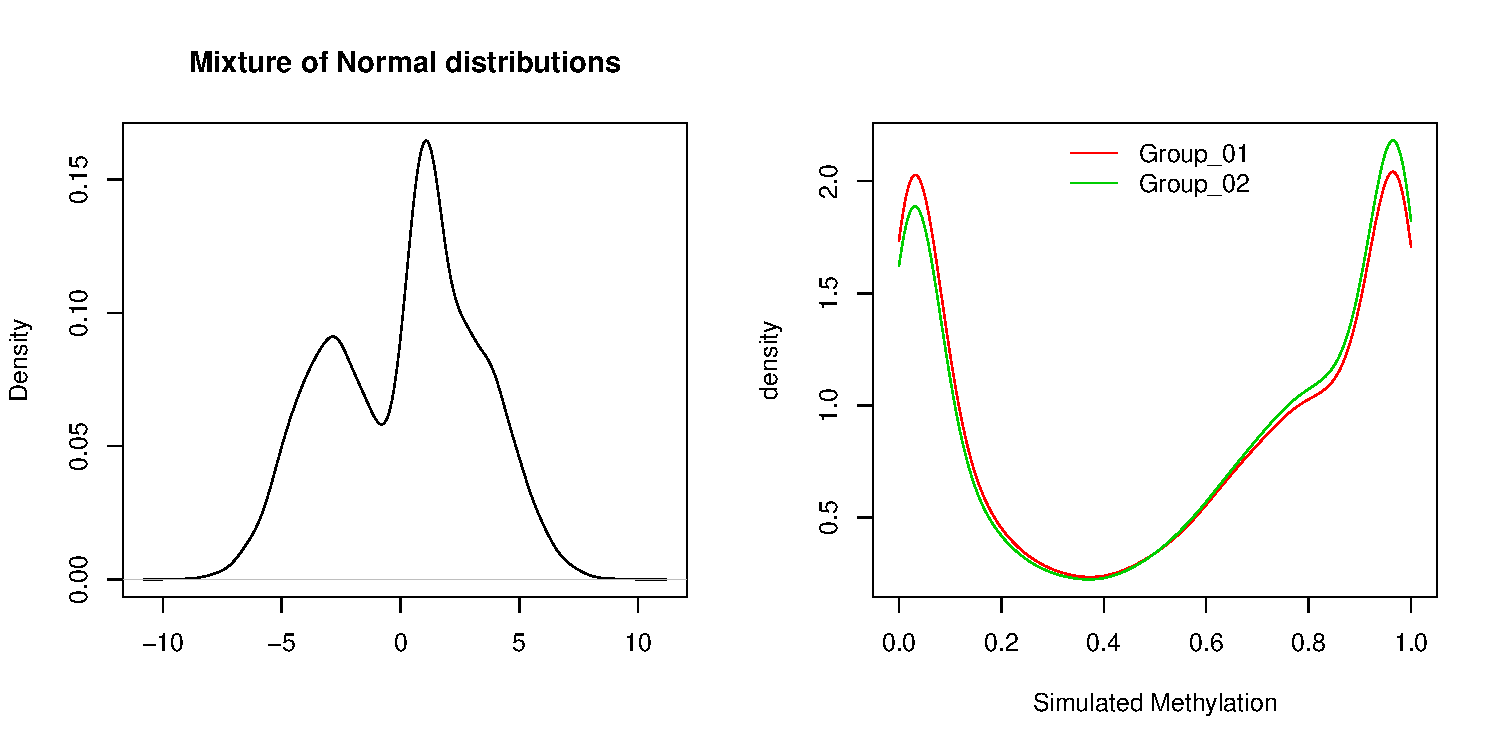
\includegraphics[width=\maxwidth]{figure/methTruth-Fig-1} 

\end{knitrout}

\texttt{pDiff} is percent of probes different relative to Group 1. If 
\texttt{nGroups} = 1, \texttt{pDiff} should be 0. If \texttt{nGroups} $>$ 1, 
the length of \texttt{pDiff} should be equal to \texttt{nGroups} - 1. The 
default for \texttt{nGroups} is 2 and the default for \texttt{pDiff} is 0.05.  

Similarly, \texttt{pUp} is proportion of \texttt{pDiff} probes that are 
methylated relative to Group 1. If \texttt{nGroups} = 1, \texttt{pUp} is 
ignored. If \texttt{nGroups} $>$ 1, the length of \texttt{pUp} should be 
equal to \texttt{nGroups} - 1.  The default for \texttt{nGroups} is 2 and 
the default for \texttt{pUp} is 0.80.

The main output will be a matrix (\texttt{methRange}) of dimension 
\texttt{nProbes} x \texttt{nGroups}. 
\begin{knitrout}
\definecolor{shadecolor}{rgb}{0.969, 0.969, 0.969}\color{fgcolor}\begin{kframe}
\begin{alltt}
\hlkwd{dim}\hlstd{(methTruth}\hlopt{$}\hlstd{methRange)}
\end{alltt}
\begin{verbatim}
## [1] 20000     2
\end{verbatim}
\end{kframe}
\end{knitrout}

The correlation between the two groups is given by:
\begin{knitrout}
\definecolor{shadecolor}{rgb}{0.969, 0.969, 0.969}\color{fgcolor}\begin{kframe}
\begin{alltt}
\hlkwd{cor}\hlstd{(methTruth}\hlopt{$}\hlstd{methRange)}
\end{alltt}
\begin{verbatim}
##           Group_01  Group_02
## Group_01 1.0000000 0.9040011
## Group_02 0.9040011 1.0000000
\end{verbatim}
\end{kframe}
\end{knitrout}

If \texttt{pDiff} was given, there will be \texttt{pDiff} $\times$ 
\texttt{nProbes} differences between the two groups. A boolean vector 
referring to which probes are different is in the \texttt{methTruth} object 
called \texttt{methDiffInd}.  Here we list the indicies of which probes 
are different between the groups: 
\begin{knitrout}
\definecolor{shadecolor}{rgb}{0.969, 0.969, 0.969}\color{fgcolor}\begin{kframe}
\begin{alltt}
\hlkwd{head}\hlstd{(}\hlkwd{which}\hlstd{(methTruth}\hlopt{$}\hlstd{methDiffInd))}
\end{alltt}
\begin{verbatim}
## [1]  53  70  86 180 186 196
\end{verbatim}
\end{kframe}
\end{knitrout}


To simulate observed DNA methylation data based on a specific technology 
platform, use the \texttt{simulateMeth} function. First, a platform from 
\texttt{list.meth.platforms} must be selected:
\begin{knitrout}
\definecolor{shadecolor}{rgb}{0.969, 0.969, 0.969}\color{fgcolor}\begin{kframe}
\begin{alltt}
\hlkwd{list.meth.platforms}\hlstd{()}
\end{alltt}
\begin{verbatim}
## [1] "methArrays"
\end{verbatim}
\end{kframe}
\end{knitrout}

Once a platform has been selected, 
\begin{knitrout}
\definecolor{shadecolor}{rgb}{0.969, 0.969, 0.969}\color{fgcolor}\begin{kframe}
\begin{alltt}
\hlkwd{set.seed}\hlstd{(}\hlnum{999}\hlstd{)}
\hlstd{simMeth} \hlkwb{<-} \hlkwd{simulateMeth}\hlstd{(methTruth,}  \hlkwc{meth.platform} \hlstd{=} \hlstr{"methArrays"}\hlstd{,}
                        \hlkwc{nSamps} \hlstd{=} \hlnum{5}\hlstd{,} \hlkwc{nMol} \hlstd{=} \hlnum{1e6}\hlstd{)}
\end{alltt}


{\ttfamily\noindent\itshape\color{messagecolor}{\#\# Simulating DNA methylation samples using the meth.platform: methArrays}}\begin{alltt}
\hlkwd{plotMeth}\hlstd{(simMeth)}
\end{alltt}
\end{kframe}
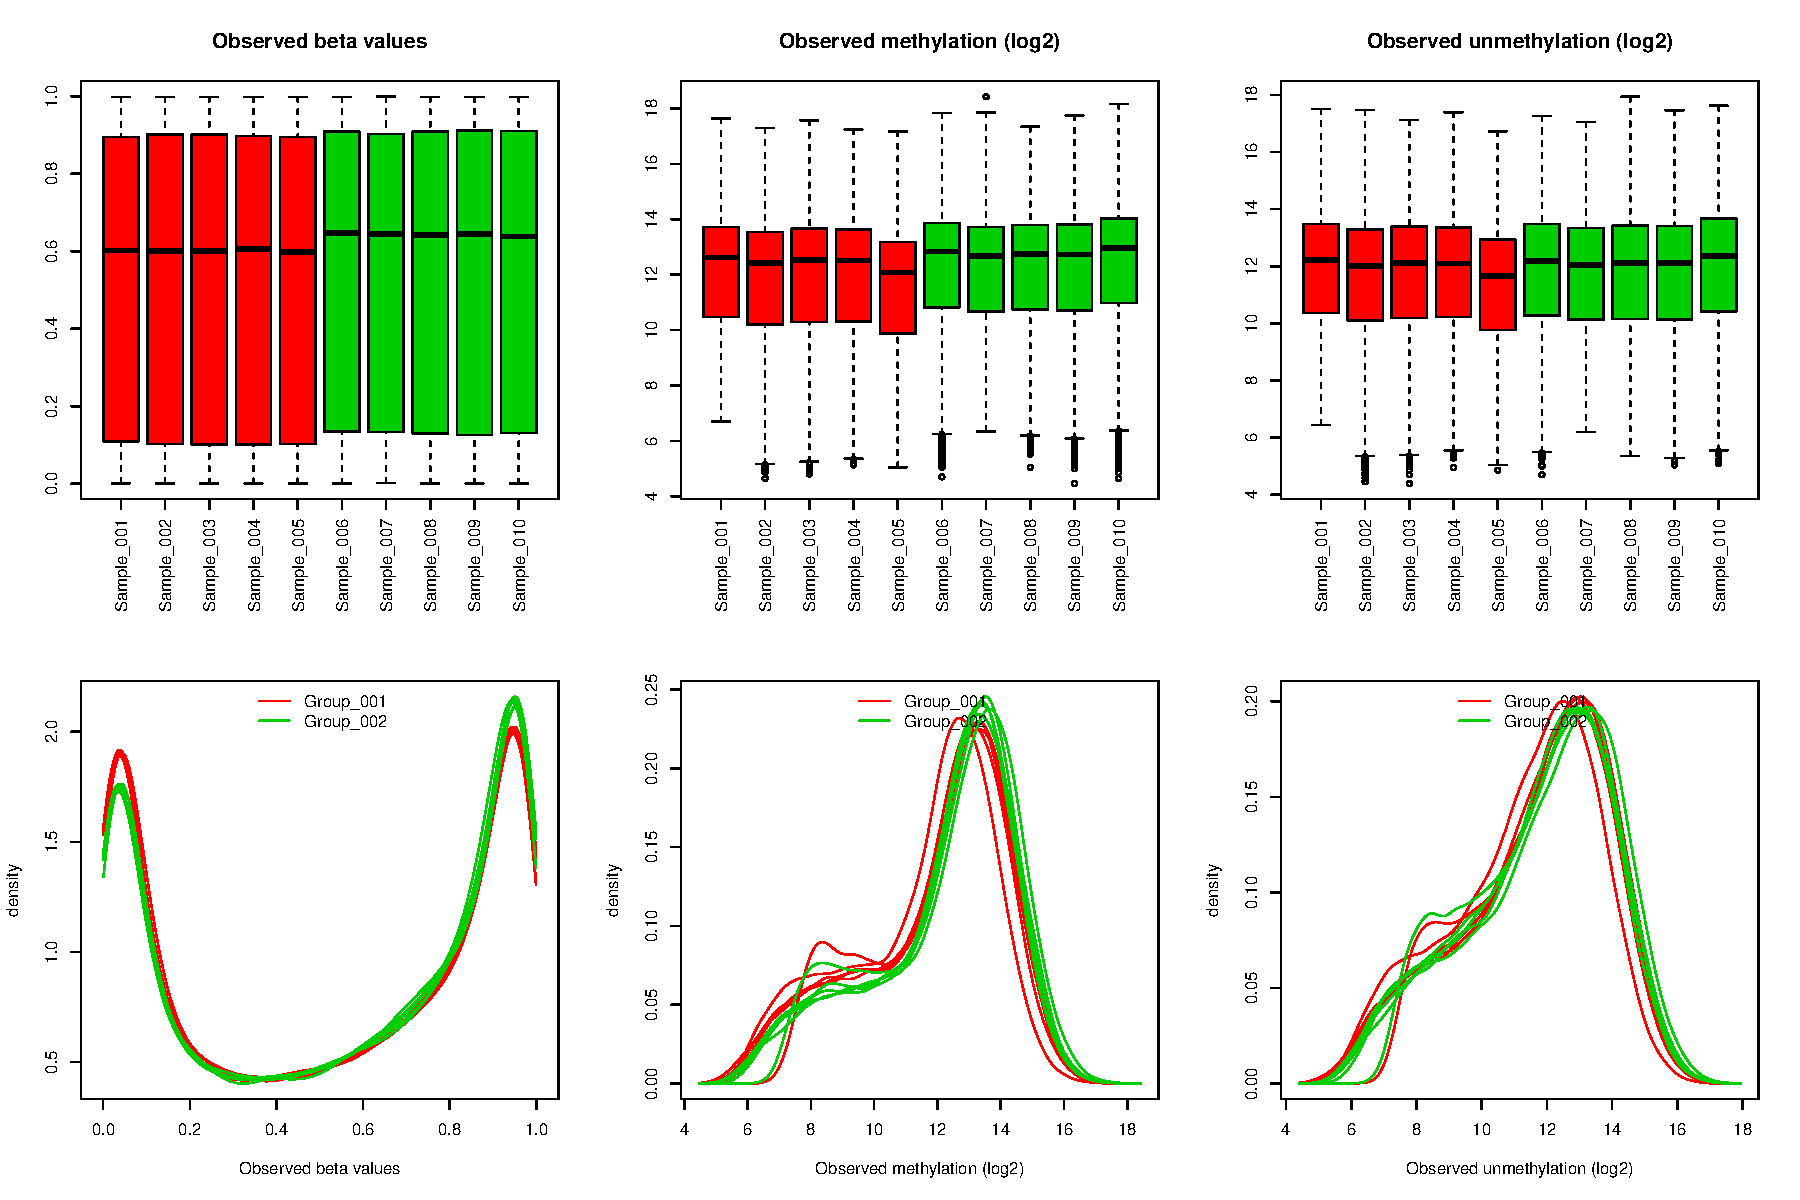
\includegraphics[width=\maxwidth]{figure/meth-figs-1} 

\end{knitrout}

\begin{knitrout}
\definecolor{shadecolor}{rgb}{0.969, 0.969, 0.969}\color{fgcolor}\begin{kframe}
\begin{alltt}
\hlkwd{summary}\hlstd{(simMeth}\hlopt{$}\hlstd{meth)}
\end{alltt}
\begin{verbatim}
##    Sample_001       Sample_002       Sample_003       Sample_004       Sample_005    
##  Min.   :   104   Min.   :    25   Min.   :    28   Min.   :    35   Min.   :    33  
##  1st Qu.:  1424   1st Qu.:  1171   1st Qu.:  1253   1st Qu.:  1270   1st Qu.:   934  
##  Median :  6293   Median :  5507   Median :  5934   Median :  5817   Median :  4329  
##  Mean   : 10007   Mean   :  8692   Mean   :  9398   Mean   :  9207   Mean   :  6786  
##  3rd Qu.: 13572   3rd Qu.: 11944   3rd Qu.: 12963   3rd Qu.: 12702   3rd Qu.:  9239  
##  Max.   :204706   Max.   :161666   Max.   :194935   Max.   :154970   Max.   :147551  
##    Sample_006       Sample_007       Sample_008       Sample_009       Sample_010    
##  Min.   :    26   Min.   :    81   Min.   :    33   Min.   :    22   Min.   :    25  
##  1st Qu.:  1809   1st Qu.:  1619   1st Qu.:  1721   1st Qu.:  1678   1st Qu.:  2006  
##  Median :  7322   Median :  6586   Median :  6912   Median :  6800   Median :  7972  
##  Mean   : 10916   Mean   :  9978   Mean   : 10459   Mean   : 10450   Mean   : 12273  
##  3rd Qu.: 14979   3rd Qu.: 13488   3rd Qu.: 14250   3rd Qu.: 14307   3rd Qu.: 16797  
##  Max.   :234445   Max.   :352368   Max.   :165850   Max.   :220224   Max.   :294473
\end{verbatim}
\end{kframe}
\end{knitrout}


\subsection{Simulating 2 or more groups}

To simulate the true level DNA methylation for a set of 2 or more groups, 
again use the the same \texttt{simulateMethTruth} function, but change 
\texttt{nGroup} and the length of \texttt{pDiff} and \texttt{pUp} 
\begin{knitrout}
\definecolor{shadecolor}{rgb}{0.969, 0.969, 0.969}\color{fgcolor}\begin{kframe}
\begin{alltt}
\hlkwd{set.seed}\hlstd{(}\hlnum{999}\hlstd{)}
\hlstd{methTruth} \hlkwb{<-} \hlkwd{simulateMethTruth}\hlstd{(}\hlkwc{nProbes} \hlstd{=} \hlnum{2e4}\hlstd{,} \hlkwc{nGroups} \hlstd{=} \hlnum{3}\hlstd{,}
                               \hlkwc{pDiff} \hlstd{=} \hlkwd{c}\hlstd{(}\hlnum{0.05}\hlstd{,} \hlnum{0.10}\hlstd{),} \hlkwc{pUp} \hlstd{=} \hlkwd{c}\hlstd{(}\hlnum{0.80}\hlstd{,} \hlnum{0.80}\hlstd{))}
\end{alltt}


{\ttfamily\noindent\itshape\color{messagecolor}{\#\# [quantroSim]: Simulating a mixture of 3 Normal distributions \\\#\#\ \ \ \ \ \ \ \ \ \ \ \  with mean (-3, 1, 3) and standard deviation (3, 0.4, 3)}}\begin{alltt}
\hlkwd{plotMethTruth}\hlstd{(methTruth)}
\end{alltt}
\end{kframe}
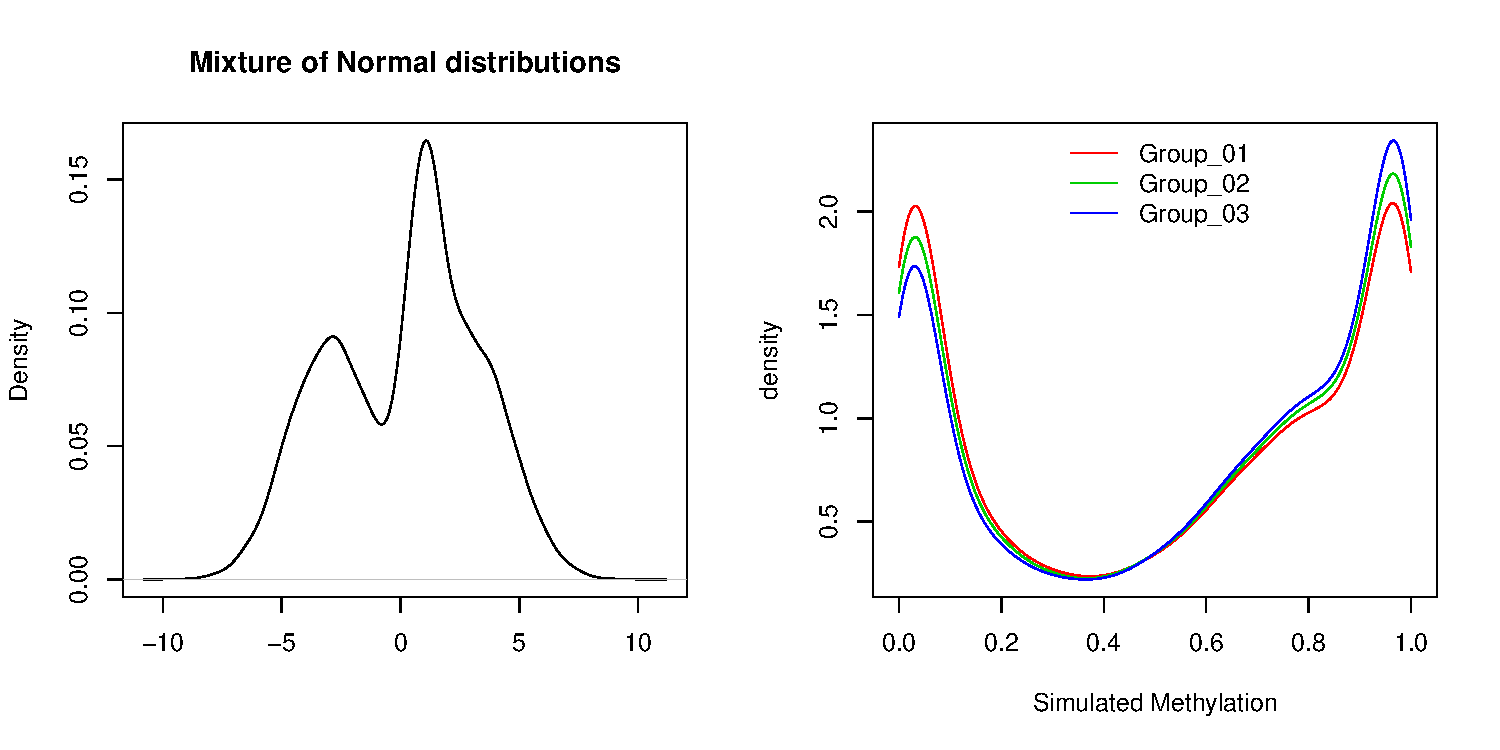
\includegraphics[width=\maxwidth]{figure/methTruth-Fig-3groups-1} 

\end{knitrout}


\begin{knitrout}
\definecolor{shadecolor}{rgb}{0.969, 0.969, 0.969}\color{fgcolor}\begin{kframe}
\begin{alltt}
\hlkwd{set.seed}\hlstd{(}\hlnum{999}\hlstd{)}
\hlstd{simMeth} \hlkwb{<-} \hlkwd{simulateMeth}\hlstd{(methTruth,}  \hlkwc{meth.platform} \hlstd{=} \hlstr{"methArrays"}\hlstd{,}
                        \hlkwc{nSamps} \hlstd{=} \hlnum{5}\hlstd{,} \hlkwc{nMol} \hlstd{=} \hlnum{1e6}\hlstd{)}
\end{alltt}


{\ttfamily\noindent\itshape\color{messagecolor}{\#\# Simulating DNA methylation samples using the meth.platform: methArrays}}\begin{alltt}
\hlkwd{plotMeth}\hlstd{(simMeth)}
\end{alltt}
\end{kframe}
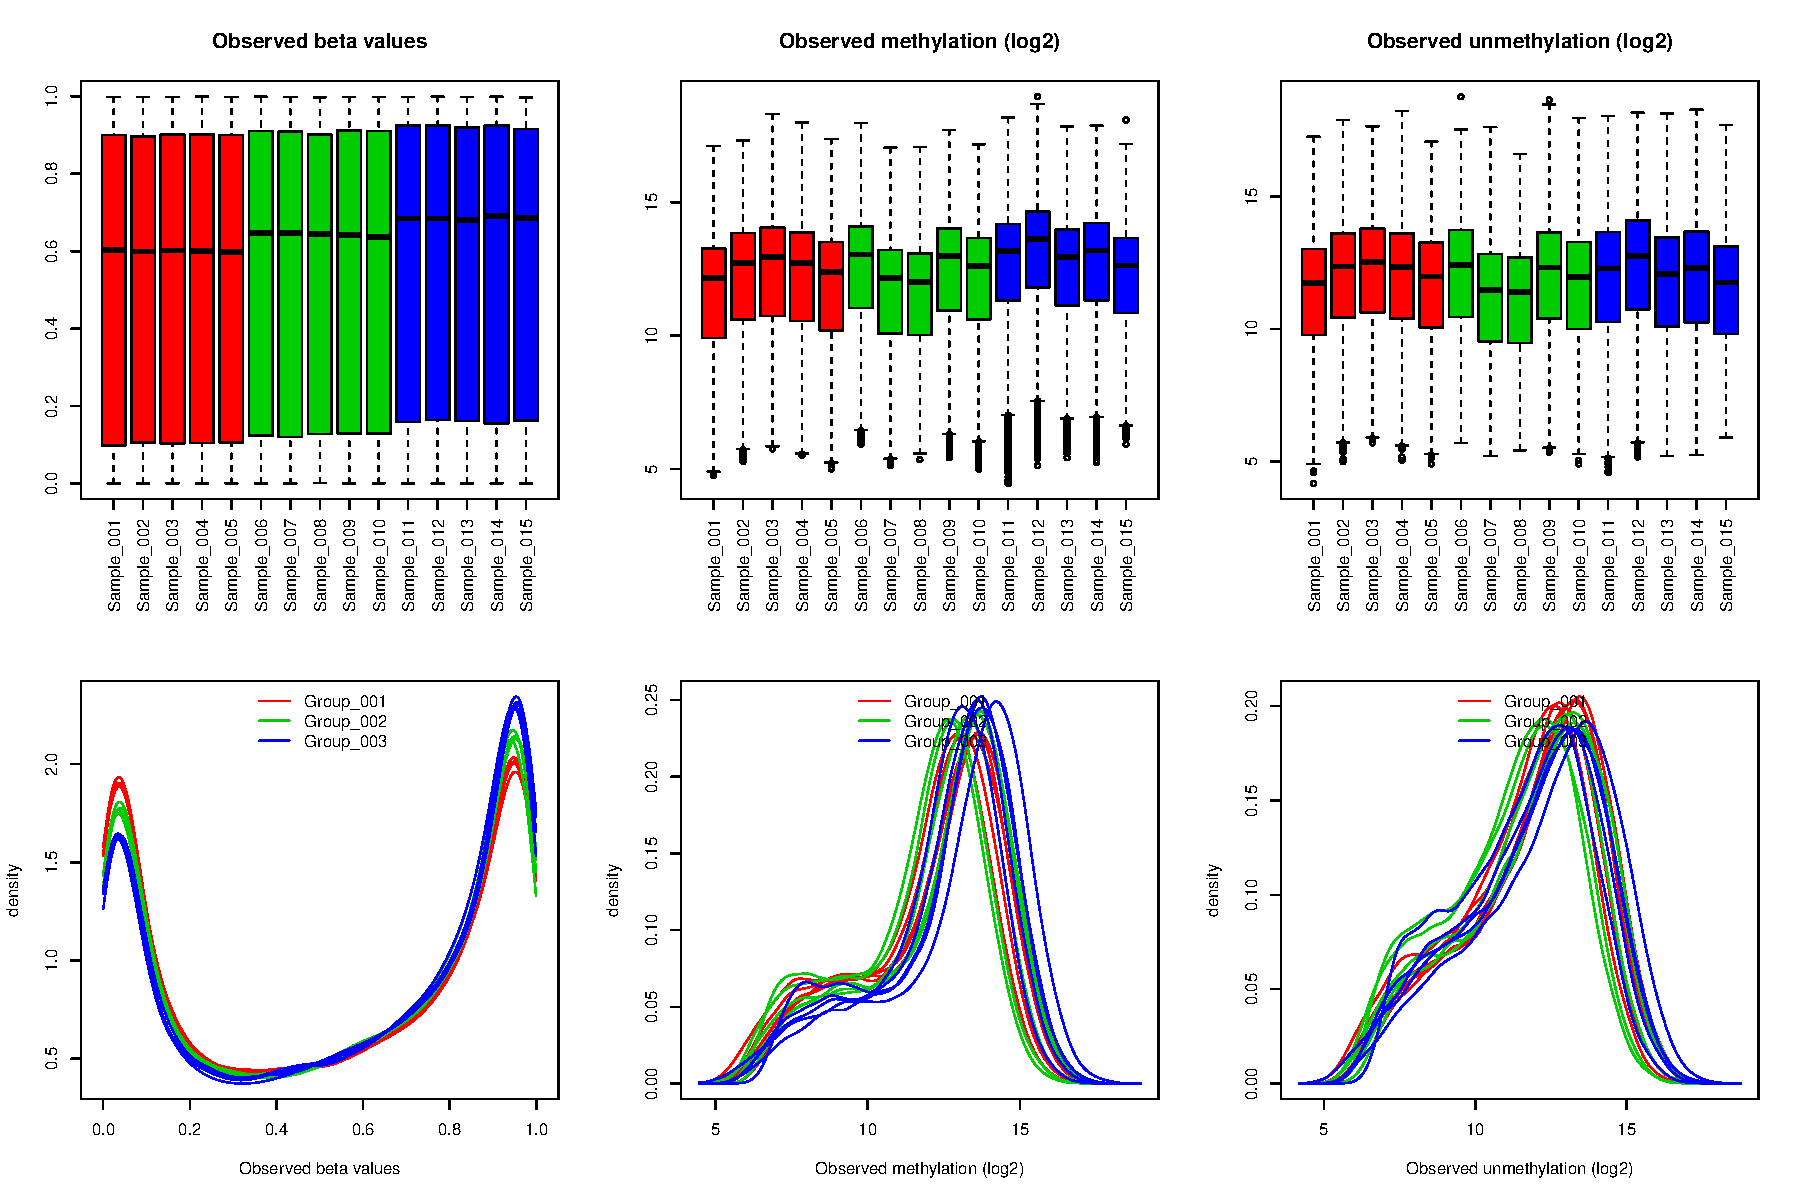
\includegraphics[width=\maxwidth]{figure/meth-figs-3groups-1} 

\end{knitrout}


\subsection{Exporting DNA Methylation arrays to the \texttt{minfi} R-package}

To export the simulated DNA methylation object to \texttt{mini}, 
use the \texttt{getMethylSet} function. 
\begin{knitrout}
\definecolor{shadecolor}{rgb}{0.969, 0.969, 0.969}\color{fgcolor}\begin{kframe}
\begin{alltt}
\hlstd{mset} \hlkwb{<-} \hlkwd{getMethylSet}\hlstd{(simMeth)}
\hlkwd{class}\hlstd{(mset)}
\end{alltt}
\begin{verbatim}
## [1] "MethylSet"
## attr(,"package")
## [1] "minfi"
\end{verbatim}
\begin{alltt}
\hlkwd{head}\hlstd{(minfi}\hlopt{::}\hlkwd{getBeta}\hlstd{(mset))}
\end{alltt}
\begin{verbatim}
##      Sample_001  Sample_002 Sample_003 Sample_004 Sample_005 Sample_006 Sample_007
## [1,] 0.00107200 0.005681153 0.02104874 0.01329519 0.00737188 0.41431311  0.7955727
## [2,] 0.60861911 0.276913189 0.70446647 0.07069987 0.37629124 0.56325955  0.2163530
## [3,] 0.07482797 0.095685249 0.01816717 0.05761364 0.09079338 0.03481271  0.1938120
## [4,] 0.70322125 0.720787152 0.83043679 0.63708213 0.54945055 0.59193881  0.8029639
## [5,] 0.99486574 0.993225380 0.99319632 0.99639552 0.97999524 0.99397809  0.9817677
## [6,] 0.23069554 0.070011669 0.02212173 0.11058865 0.05687072 0.24056654  0.3724013
##      Sample_008 Sample_009 Sample_010 Sample_011  Sample_012  Sample_013  Sample_014
## [1,]  0.7364314 0.91680635 0.77712990 0.02488748 0.002076259 0.005362042 0.004826758
## [2,]  0.8182779 0.52998079 0.39585037 0.17606363 0.120002272 0.663642288 0.300044929
## [3,]  0.0851244 0.01245816 0.06346039 0.02830494 0.207956104 0.036411478 0.004687271
## [4,]  0.3784451 0.55584783 0.76532300 0.64324741 0.754493350 0.759291671 0.719616451
## [5,]  0.9953099 0.99766246 0.96271244 0.99657460 0.996118589 0.991937581 0.991931844
## [6,]  0.1335530 0.19840104 0.08672005 0.09554162 0.531417351 0.059207410 0.167966442
##      Sample_015
## [1,] 0.01559584
## [2,] 0.20763109
## [3,] 0.03816986
## [4,] 0.74108434
## [5,] 0.98429578
## [6,] 0.35855504
\end{verbatim}
\end{kframe}
\end{knitrout}

Functions in the \texttt{minfi} R/Bioconductor package such as \texttt{getBeta}, \texttt{getM}, \texttt{getCN} can be used after creating a \texttt{MethylSet} with the function \texttt{getMethylSet}. 

Note: there is no manifest and no method was used to preprocess the 
simulated data. Therefore, these functions from \texttt{minfi} will not work.  
\begin{knitrout}
\definecolor{shadecolor}{rgb}{0.969, 0.969, 0.969}\color{fgcolor}\begin{kframe}
\begin{alltt}
\hlkwd{getManifest}\hlstd{(mset)}
\hlkwd{preprocessMethod}\hlstd{(mset)}
\end{alltt}
\end{kframe}
\end{knitrout}

\subsection{Additional options for \texttt{simulateMeth}}

\subsubsection{Controlling level of technical variation}
We use the Langmuir model to simulate chemical saturation observed using 
microarrays. Our model to simulate raw methylation and unmethylation value 
for the $j^{th}$ probe from the $i^{th}$ sample in the $k^{th}$ group is 
given by
\[ M_{ijk} = o_{ijk} + d_{ijk} + a_{ijk} ( \frac{x_{jk}^m}{x_{jk}^m + b_{ijk}} ) \epsilon_{ijk} \]
\[ U_{ijk} = o_{ijk} + d_{ijk} + a_{ijk}  ( \frac{x_{jk}^u}{x_{jk}^u + b_{ijk}} ) \epsilon_{ijk} \]
where $x_{jk}^m$ and $x_{jk}^u$ are the expected number of methylated and 
unmethylated molecules at $j^{th}$ probe in the $k^{th}$ group and the rest 
are parameters simulated from a log Normal distribution with a given set of 
hyperparameters. For example, $a_{ijk} = a_{ik} * a_j$ represents the 
florescence intensity from the scanner. We define $a_{ijk} = a_{ik} * a_j$ 
and let both parameters $a_{ik}$ (sample-level noise) and $a_j$ 
(probe-level noise) each have their own hyperparameters to allow for 
global shifts: 
\[ \log_2(a_{ik}) \sim  N(16, 0.1) \]
\[ \log_2(a_{j}) \sim N(0, 0.01)  \]

Similarly, $b_{ijk} = b_{ik} * b_j$ and $o_{ijk} = o_{ik} * o_j$ 
(optical noise) where the sample-level noise is simulated using
\[ \log_2(b_{ik}) \sim  N(22, 0.1) \]
\[ \log_2(o_{ik}) \sim  N(5, 1) \]
\[ \log_2(d_{ijk}) \sim  N(5, 1) \]
\[ \log_2(\epsilon_{ijk}) \sim  N(0, 1) \]

For efficiency, we simulate the parameters from a multivariate normal 
distribution for all 10 arrays (=5 samples per group * 2 groups). In the 
above example, covariance matrices would be given by:
\begin{knitrout}
\definecolor{shadecolor}{rgb}{0.969, 0.969, 0.969}\color{fgcolor}\begin{kframe}
\begin{alltt}
\hlkwd{set.seed}\hlstd{(}\hlnum{999}\hlstd{)}
\hlstd{siga} \hlkwb{=} \hlstd{sigb} \hlkwb{=} \hlnum{0.1} \hlopt{*} \hlkwd{diag}\hlstd{(}\hlnum{10}\hlstd{)}
\hlstd{sigOpt} \hlkwb{=} \hlnum{1} \hlopt{*} \hlkwd{diag}\hlstd{(}\hlnum{10}\hlstd{)}

\hlstd{methTruth} \hlkwb{<-} \hlkwd{simulateMethTruth}\hlstd{(}\hlkwc{nProbes} \hlstd{=} \hlnum{2e4}\hlstd{,} \hlkwc{nGroups} \hlstd{=} \hlnum{2}\hlstd{,}
                               \hlkwc{pDiff} \hlstd{=} \hlnum{0.05}\hlstd{,} \hlkwc{pUp} \hlstd{=} \hlnum{0.80}\hlstd{)}
\end{alltt}


{\ttfamily\noindent\itshape\color{messagecolor}{\#\# [quantroSim]: Simulating a mixture of 3 Normal distributions \\\#\#\ \ \ \ \ \ \ \ \ \ \ \  with mean (-3, 1, 3) and standard deviation (3, 0.4, 3)}}\begin{alltt}
\hlstd{simMeth} \hlkwb{<-} \hlkwd{simulateMeth}\hlstd{(methTruth,}  \hlkwc{meth.platform} \hlstd{=} \hlstr{"methArrays"}\hlstd{,}
                        \hlkwc{nSamps} \hlstd{=} \hlnum{5}\hlstd{,} \hlkwc{nMol} \hlstd{=} \hlnum{1e6}\hlstd{,}
                        \hlkwc{siga} \hlstd{= siga,} \hlkwc{sigb} \hlstd{= sigb,} \hlkwc{sigOpt} \hlstd{= sigOpt)}
\end{alltt}


{\ttfamily\noindent\itshape\color{messagecolor}{\#\# Simulating DNA methylation samples using the meth.platform: methArrays}}\begin{alltt}
\hlkwd{plotMeth}\hlstd{(simMeth)}
\end{alltt}
\end{kframe}
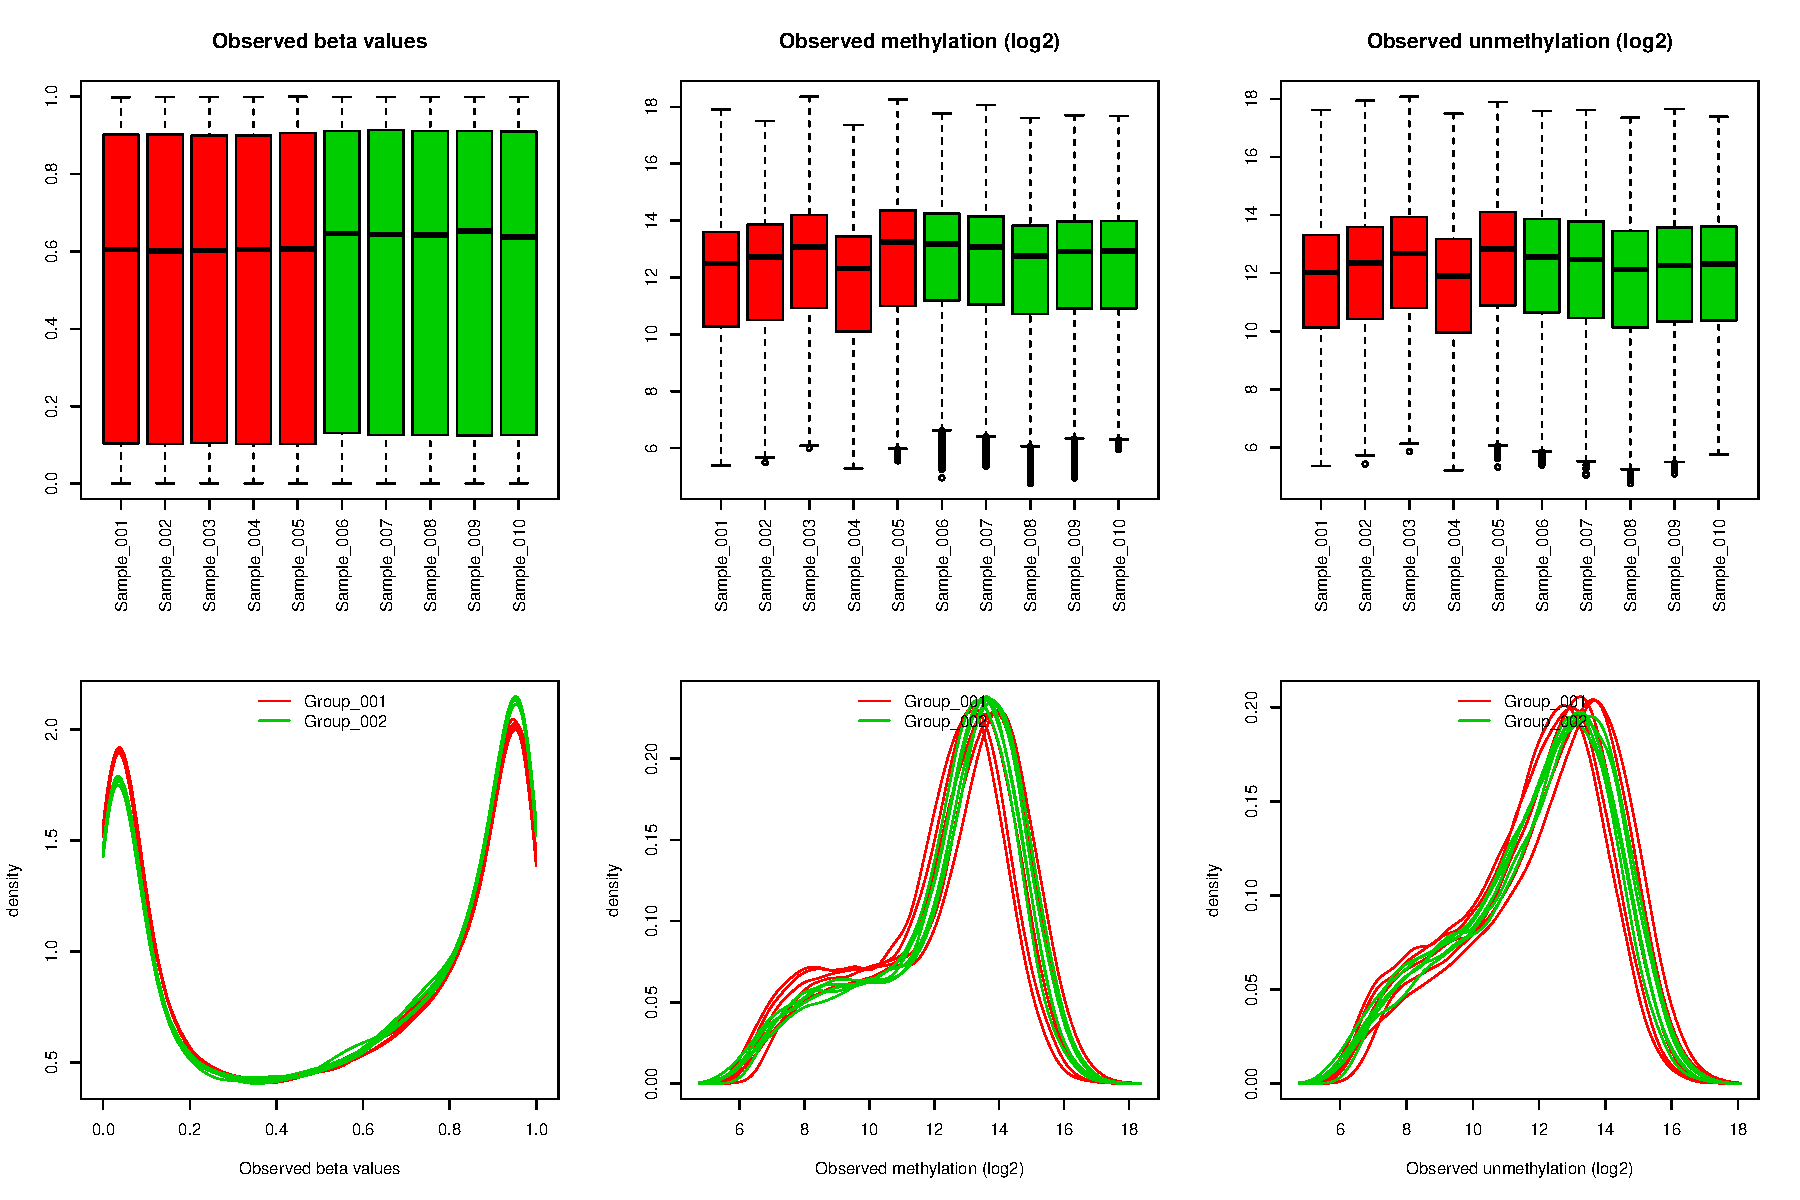
\includegraphics[width=\maxwidth]{figure/simMeth-figs2-1} 

\end{knitrout}
These are the default values for the (\texttt{siga}, \texttt{sigb} 
and \texttt{sibOpt}) parameters in the \texttt{simulateMeth} function. 

To control how much technical variation is induced from the 
platform-technology, the variance hyperparameters from the sample-level 
noise (\texttt{siga}, \texttt{sigb} and \texttt{sibOpt}) can be 
controlled manually.
\begin{knitrout}
\definecolor{shadecolor}{rgb}{0.969, 0.969, 0.969}\color{fgcolor}\begin{kframe}
\begin{alltt}
\hlkwd{set.seed}\hlstd{(}\hlnum{999}\hlstd{)}
\hlstd{siga} \hlkwb{=} \hlstd{sigb} \hlkwb{=} \hlnum{1} \hlopt{*} \hlkwd{diag}\hlstd{(}\hlnum{10}\hlstd{)}
\hlstd{sigOpt} \hlkwb{=} \hlnum{2} \hlopt{*} \hlkwd{diag}\hlstd{(}\hlnum{10}\hlstd{)}
\hlstd{simMeth} \hlkwb{<-} \hlkwd{simulateMeth}\hlstd{(methTruth,}  \hlkwc{meth.platform} \hlstd{=} \hlstr{"methArrays"}\hlstd{,}
                        \hlkwc{nSamps} \hlstd{=} \hlnum{5}\hlstd{,} \hlkwc{nMol} \hlstd{=} \hlnum{1e6}\hlstd{,}
                        \hlkwc{siga} \hlstd{= siga,} \hlkwc{sigb} \hlstd{= sigb,} \hlkwc{sigOpt} \hlstd{= sigOpt)}
\end{alltt}


{\ttfamily\noindent\itshape\color{messagecolor}{\#\# Simulating DNA methylation samples using the meth.platform: methArrays}}\begin{alltt}
\hlkwd{plotMeth}\hlstd{(simMeth)}
\end{alltt}
\end{kframe}
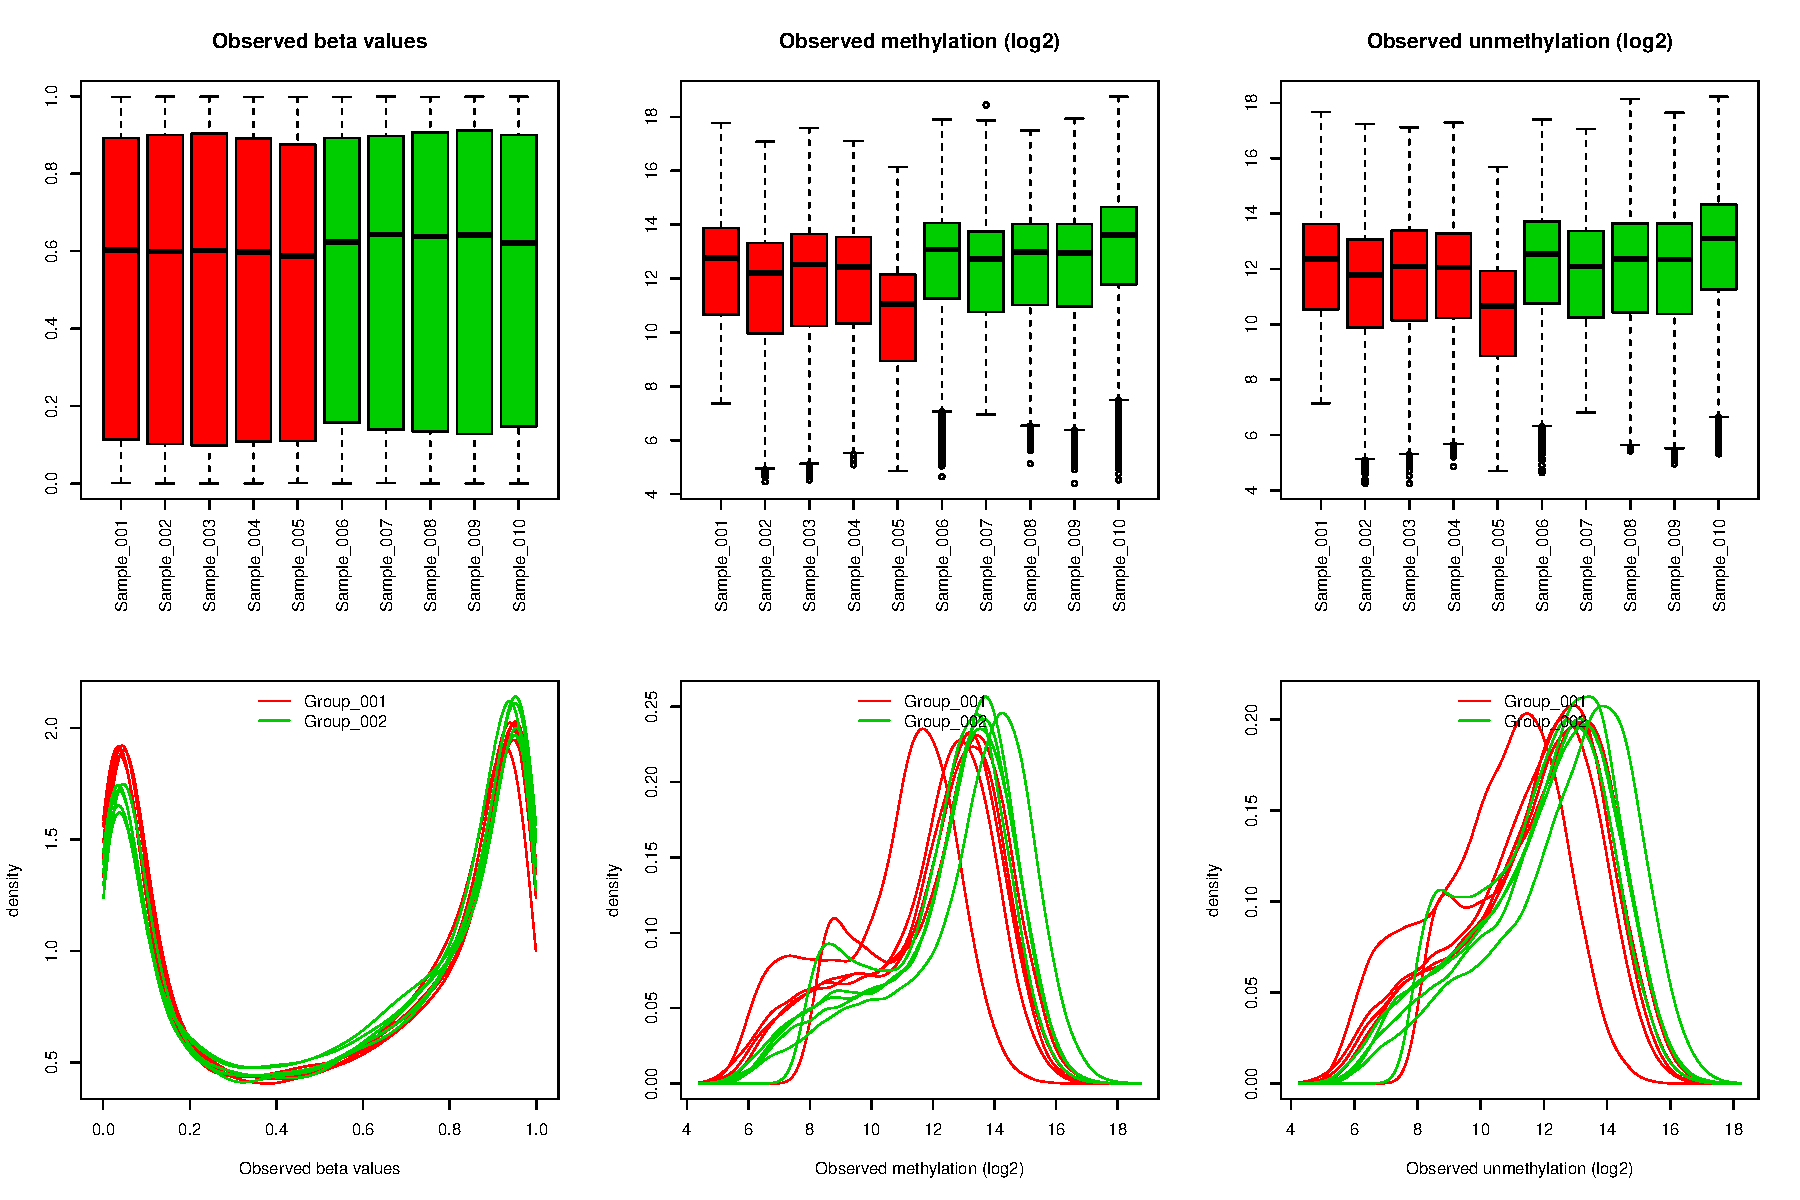
\includegraphics[width=\maxwidth]{figure/simMeth-figs3-1} 

\end{knitrout}







\section{Gene Expression}
There are two main functions used to generate simulated gene expression data: 
\texttt{simulateGExTruth} and \texttt{simulateGEx}. The first function 
(\texttt{simulateGExTruth}) generates the true gene expression without any 
consideration for a platform technology. The second function 
(\texttt{simulateGEx}) simulates observed gene expression based on: 

\begin{enumerate}
\item the platform technology 
\item the magnitude of technical variation
\end{enumerate}


\subsection{Quick Start}
To simulate the true level gene expression for a set of 2 groups, use the 
\texttt{simulateGExTruth} function. 
\begin{knitrout}
\definecolor{shadecolor}{rgb}{0.969, 0.969, 0.969}\color{fgcolor}\begin{kframe}
\begin{alltt}
\hlkwd{set.seed}\hlstd{(}\hlnum{999}\hlstd{)}
\hlstd{geneTruth} \hlkwb{<-} \hlkwd{simulateGExTruth}\hlstd{(}\hlkwc{nGenes} \hlstd{=} \hlnum{2e4}\hlstd{,} \hlkwc{nGroups} \hlstd{=} \hlnum{2}\hlstd{,}
                              \hlkwc{pDiff} \hlstd{=} \hlnum{0.05}\hlstd{,} \hlkwc{foldDiff} \hlstd{=} \hlnum{5}\hlstd{)}
\end{alltt}


{\ttfamily\noindent\itshape\color{messagecolor}{\#\# [quantroSim]: Simulating RNA transcript counts using a Poisson \\\#\#\ \ \ \ \ \ \ \ \ \  distribution with mean parameters from 0.01 to 4662.66}}\begin{alltt}
\hlkwd{plotGExTruth}\hlstd{(geneTruth)}
\end{alltt}
\end{kframe}
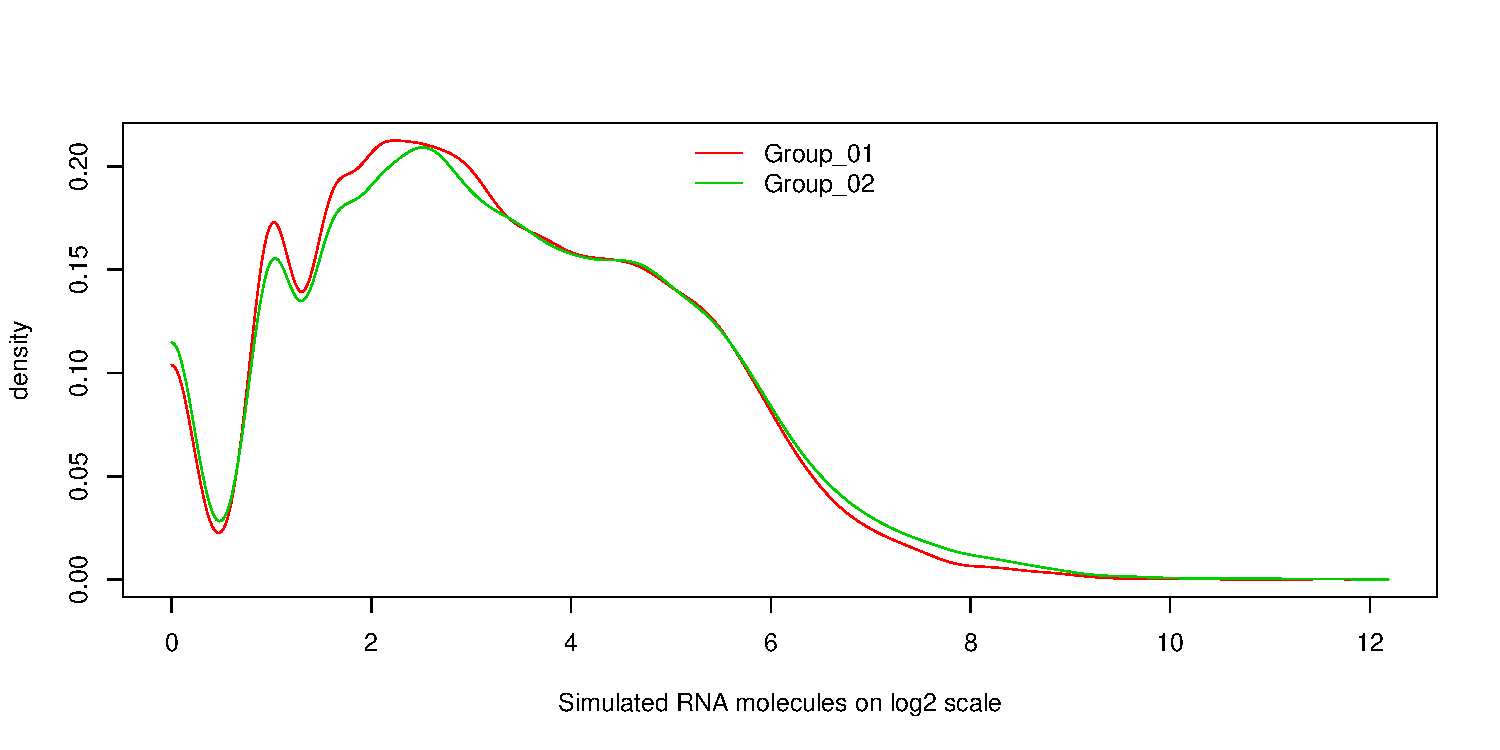
\includegraphics[width=\maxwidth]{figure/geneTruth-Fig-1} 

\end{knitrout}

Similar to \texttt{simulateMethTruth}, \texttt{pDiff} is percent of probes 
different relative to Group 1. If \texttt{nGroups} = 1, \texttt{pDiff} 
should be 0. If \texttt{nGroups} $>$ 1, the length of \texttt{pDiff} should 
be equal to \texttt{nGroups} - 1. The default for \texttt{nGroups} is 2 and 
the default for \texttt{pDiff} is 0.05.  

\texttt{foldDiff} is the fold difference of gene differentially expressed in 
one group relative to Group 1. If \texttt{nGroups} = 1, \texttt{foldDiff} is 
ignored. If \texttt{nGroups} $>$ 1, the length of \texttt{foldDiff} should be 
equal to \texttt{nGroups} - 1.  The default for \texttt{nGroups} is 2 and 
the default for \texttt{foldDiff} is 5.

The main output will be a matrix (\texttt{geneRange}) of dimension 
\texttt{nGenes} x \texttt{nGroups}. 
\begin{knitrout}
\definecolor{shadecolor}{rgb}{0.969, 0.969, 0.969}\color{fgcolor}\begin{kframe}
\begin{alltt}
\hlkwd{dim}\hlstd{(geneTruth}\hlopt{$}\hlstd{geneRange)}
\end{alltt}
\begin{verbatim}
## [1] 20000     2
\end{verbatim}
\end{kframe}
\end{knitrout}

The correlation between the two groups is given by:
\begin{knitrout}
\definecolor{shadecolor}{rgb}{0.969, 0.969, 0.969}\color{fgcolor}\begin{kframe}
\begin{alltt}
\hlkwd{cor}\hlstd{(geneTruth}\hlopt{$}\hlstd{geneRange)}
\end{alltt}
\begin{verbatim}
##           Group_01  Group_02
## Group_01 1.0000000 0.8736777
## Group_02 0.8736777 1.0000000
\end{verbatim}
\end{kframe}
\end{knitrout}

If \texttt{pDiff} was given, there will be \texttt{pDiff} $\times$ 
\texttt{nGenes} differences between the two groups. A boolean vector 
referring to which genes are different is in the \texttt{geneTruth} object 
called \texttt{genesDiffInd}.  Here we list the indicies of which genes 
are different between the groups: 
\begin{knitrout}
\definecolor{shadecolor}{rgb}{0.969, 0.969, 0.969}\color{fgcolor}\begin{kframe}
\begin{alltt}
\hlkwd{head}\hlstd{(}\hlkwd{which}\hlstd{(geneTruth}\hlopt{$}\hlstd{genesDiffInd))}
\end{alltt}
\begin{verbatim}
## [1]  28  43  67  85 117 130
\end{verbatim}
\end{kframe}
\end{knitrout}


To simulate observed gene expression data based on a specific technology 
platform, use the \texttt{simulateGEx} function. First, a platform from 
\texttt{list.GEx.platforms} must be selected:
\begin{knitrout}
\definecolor{shadecolor}{rgb}{0.969, 0.969, 0.969}\color{fgcolor}\begin{kframe}
\begin{alltt}
\hlkwd{list.GEx.platforms}\hlstd{()}
\end{alltt}
\begin{verbatim}
## [1] "GExArrays"
\end{verbatim}
\end{kframe}
\end{knitrout}

Once a platform has been selected, 
\begin{knitrout}
\definecolor{shadecolor}{rgb}{0.969, 0.969, 0.969}\color{fgcolor}\begin{kframe}
\begin{alltt}
\hlkwd{set.seed}\hlstd{(}\hlnum{999}\hlstd{)}
\hlstd{sim} \hlkwb{<-} \hlkwd{simulateGEx}\hlstd{(geneTruth,}  \hlkwc{GEx.platform} \hlstd{=} \hlstr{"GExArrays"}\hlstd{,} \hlkwc{nSamps} \hlstd{=} \hlnum{5}\hlstd{)}
\end{alltt}


{\ttfamily\noindent\itshape\color{messagecolor}{\#\# Simulating gene expression samples using the GEx.platform: GExArrays\\\#\# No PCR amplification of RNA transcript counts.}}\begin{alltt}
\hlkwd{plotGEx}\hlstd{(sim)}
\end{alltt}
\end{kframe}
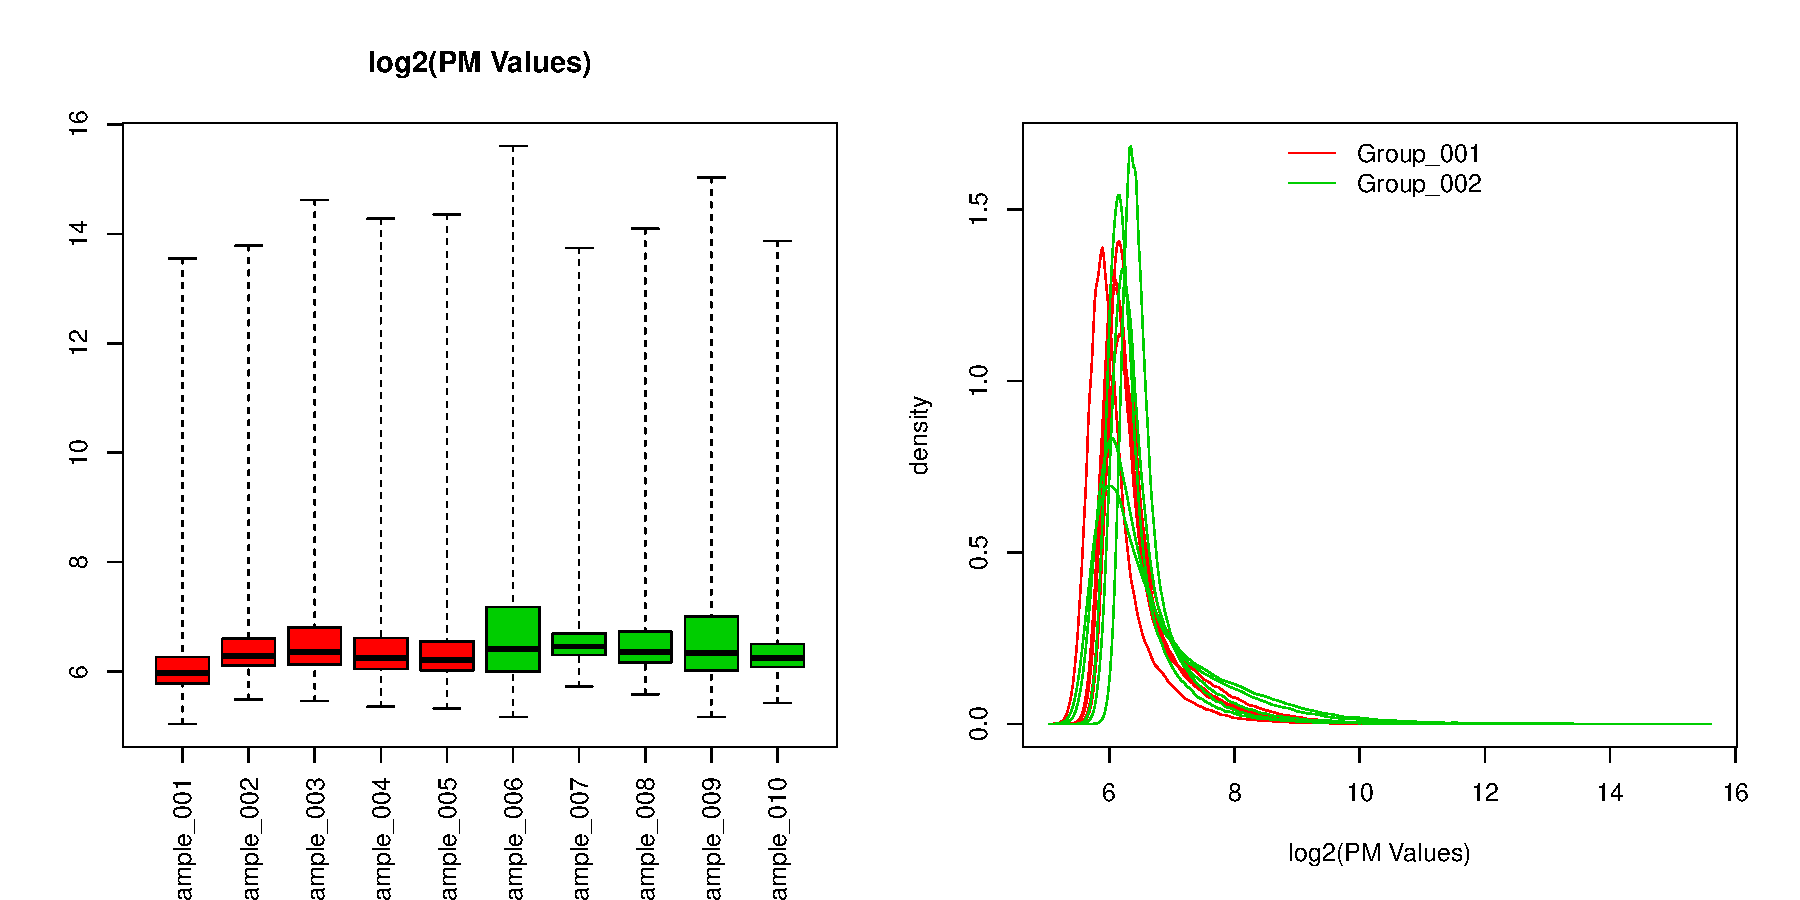
\includegraphics[width=\maxwidth]{figure/gene-figs-1} 

\end{knitrout}

\begin{knitrout}
\definecolor{shadecolor}{rgb}{0.969, 0.969, 0.969}\color{fgcolor}\begin{kframe}
\begin{alltt}
\hlkwd{summary}\hlstd{(simMeth}\hlopt{$}\hlstd{meth)}
\end{alltt}
\begin{verbatim}
##    Sample_001       Sample_002       Sample_003       Sample_004       Sample_005   
##  Min.   :   165   Min.   :    22   Min.   :    23   Min.   :    34   Min.   :   29  
##  1st Qu.:  1614   1st Qu.:  1002   1st Qu.:  1214   1st Qu.:  1281   1st Qu.:  493  
##  Median :  6986   Median :  4710   Median :  5884   Median :  5522   Median : 2146  
##  Mean   : 11110   Mean   :  7431   Mean   :  9363   Mean   :  8658   Mean   : 3339  
##  3rd Qu.: 15055   3rd Qu.: 10206   3rd Qu.: 12929   3rd Qu.: 11959   3rd Qu.: 4529  
##  Max.   :224914   Max.   :138133   Max.   :197185   Max.   :141540   Max.   :71803  
##    Sample_006       Sample_007       Sample_008       Sample_009       Sample_010    
##  Min.   :    25   Min.   :   124   Min.   :    35   Min.   :    21   Min.   :    23  
##  1st Qu.:  2455   1st Qu.:  1724   1st Qu.:  2081   1st Qu.:  1994   1st Qu.:  3531  
##  Median :  8626   Median :  6742   Median :  8086   Median :  7930   Median : 12504  
##  Mean   : 12532   Mean   : 10165   Mean   : 12157   Mean   : 12134   Mean   : 18862  
##  3rd Qu.: 17090   3rd Qu.: 13719   3rd Qu.: 16570   3rd Qu.: 16652   3rd Qu.: 25760  
##  Max.   :244585   Max.   :355651   Max.   :185149   Max.   :250245   Max.   :440915
\end{verbatim}
\end{kframe}
\end{knitrout}





\subsection{Simulating 2 or more groups}

To simulate the true level gene expression for a set of 2 or more groups, 
again use the the same \texttt{simulateGExTruth} function, but change 
\texttt{nGroup} and the length of \texttt{pDiff} and \texttt{foldDiff} 
\begin{knitrout}
\definecolor{shadecolor}{rgb}{0.969, 0.969, 0.969}\color{fgcolor}\begin{kframe}
\begin{alltt}
\hlkwd{set.seed}\hlstd{(}\hlnum{999}\hlstd{)}
\hlstd{geneTruth} \hlkwb{<-} \hlkwd{simulateGExTruth}\hlstd{(}\hlkwc{nGenes} \hlstd{=} \hlnum{2e4}\hlstd{,} \hlkwc{nGroups} \hlstd{=} \hlnum{3}\hlstd{,}
                              \hlkwc{pDiff} \hlstd{=} \hlkwd{c}\hlstd{(}\hlnum{0.05}\hlstd{,} \hlnum{0.10}\hlstd{),} \hlkwc{foldDiff} \hlstd{=} \hlkwd{c}\hlstd{(}\hlnum{5}\hlstd{,}\hlnum{5}\hlstd{))}
\end{alltt}


{\ttfamily\noindent\itshape\color{messagecolor}{\#\# [quantroSim]: Simulating RNA transcript counts using a Poisson \\\#\#\ \ \ \ \ \ \ \ \ \  distribution with mean parameters from 0.01 to 4662.66}}\begin{alltt}
\hlkwd{plotGExTruth}\hlstd{(geneTruth)}
\end{alltt}
\end{kframe}
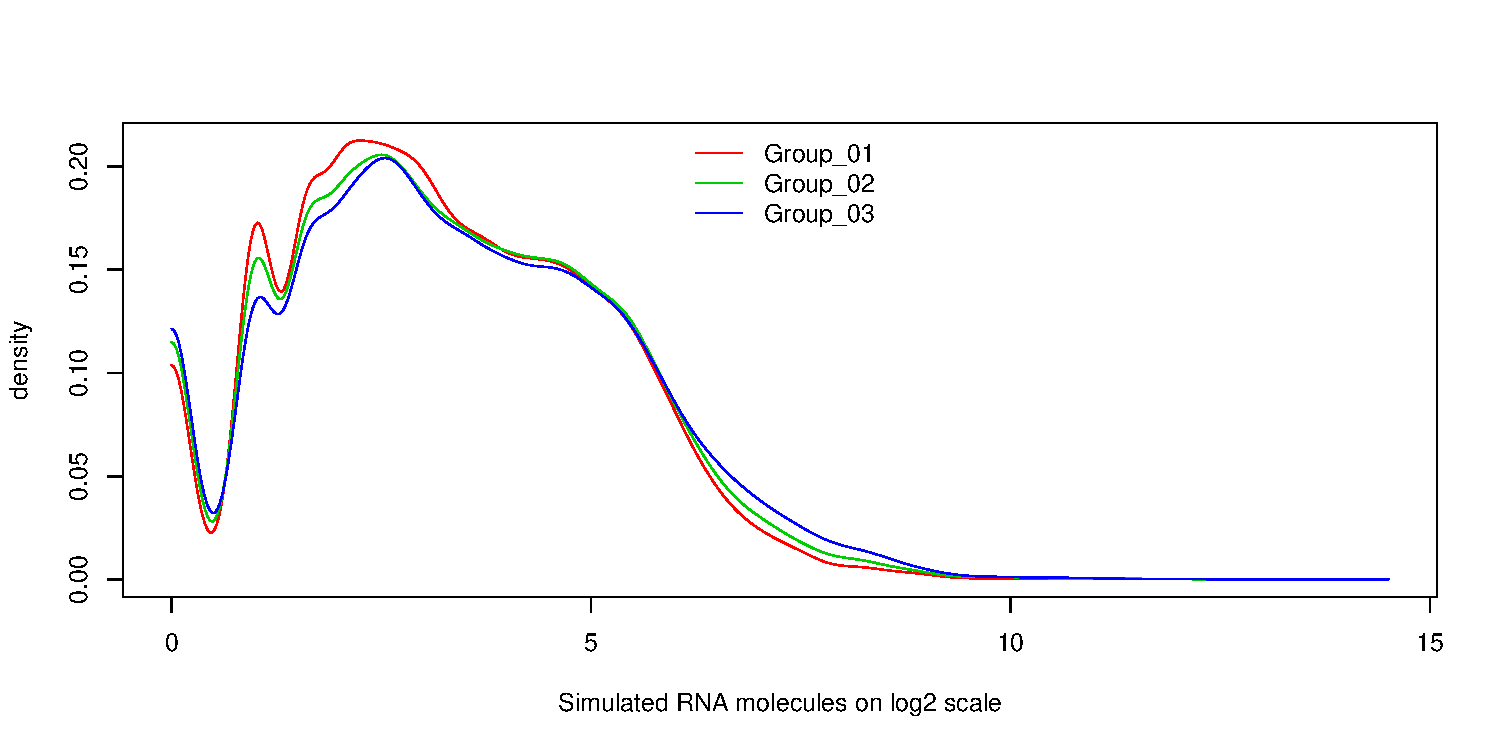
\includegraphics[width=\maxwidth]{figure/geneTruth-Fig-3groups-1} 

\end{knitrout}


\begin{knitrout}
\definecolor{shadecolor}{rgb}{0.969, 0.969, 0.969}\color{fgcolor}\begin{kframe}
\begin{alltt}
\hlkwd{set.seed}\hlstd{(}\hlnum{999}\hlstd{)}
\hlstd{sim} \hlkwb{<-} \hlkwd{simulateGEx}\hlstd{(geneTruth,}  \hlkwc{GEx.platform} \hlstd{=} \hlstr{"GExArrays"}\hlstd{,} \hlkwc{nSamps} \hlstd{=} \hlnum{5}\hlstd{)}
\end{alltt}


{\ttfamily\noindent\itshape\color{messagecolor}{\#\# Simulating gene expression samples using the GEx.platform: GExArrays\\\#\# No PCR amplification of RNA transcript counts.}}\begin{alltt}
\hlkwd{plotGEx}\hlstd{(sim)}
\end{alltt}
\end{kframe}
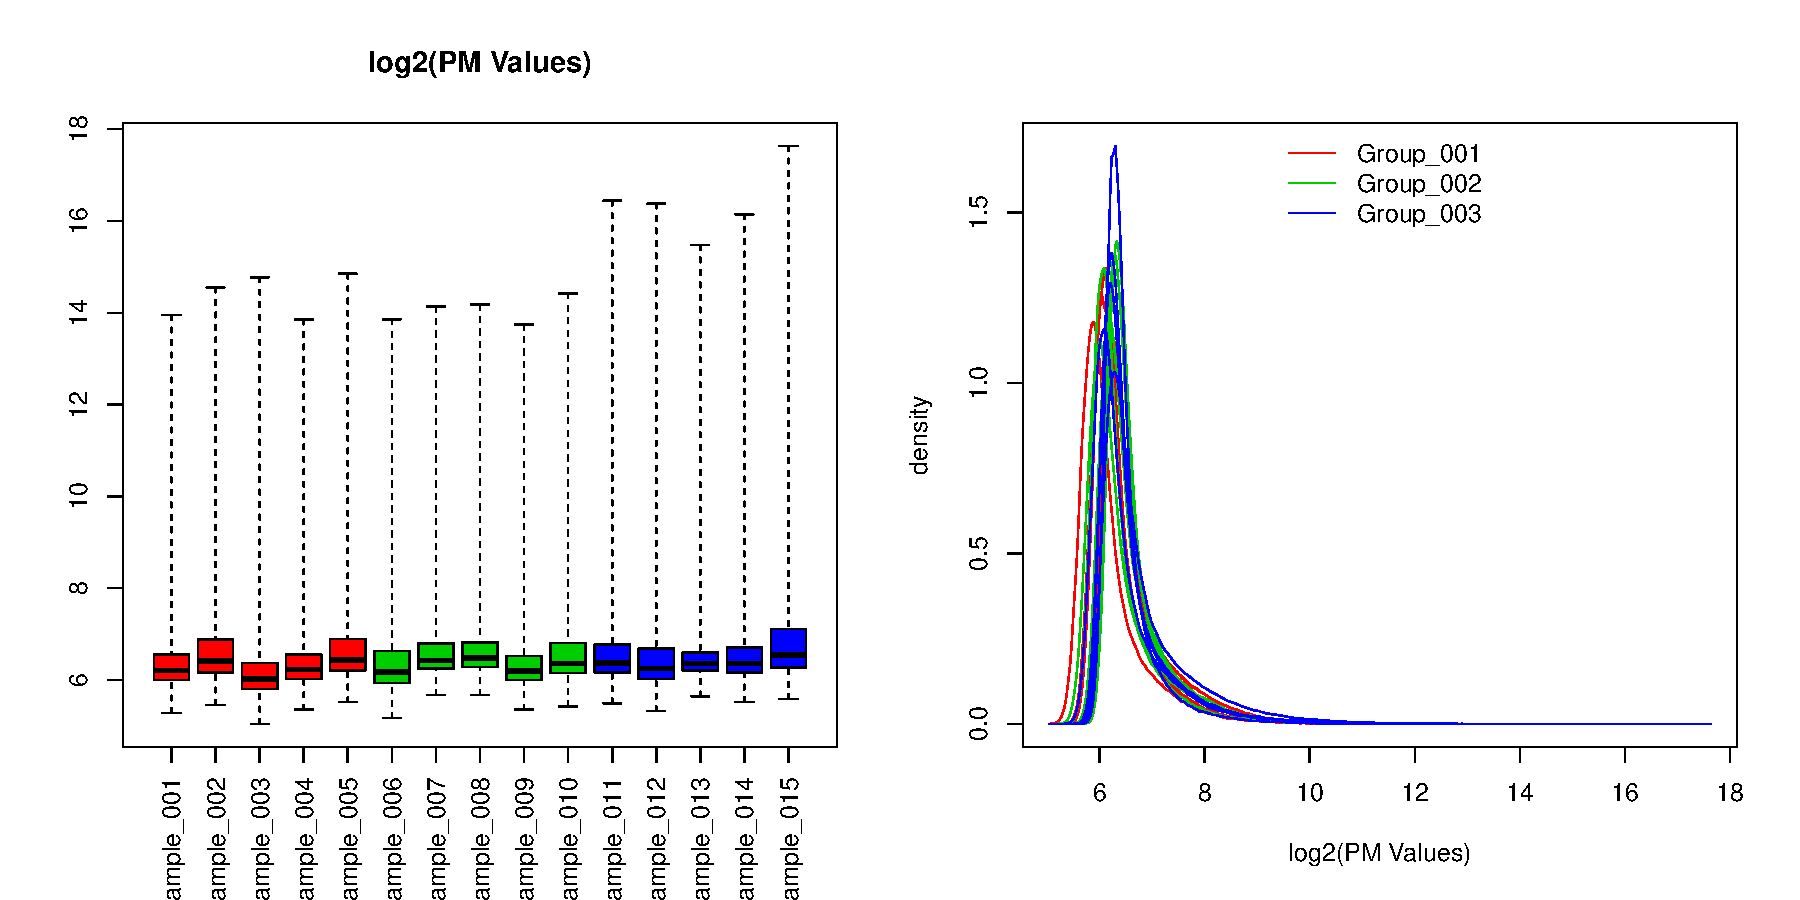
\includegraphics[width=\maxwidth]{figure/gene-figs-3groups-1} 

\end{knitrout}




\subsection{Additional options for \texttt{simulateGEx}}

\subsubsection{Controlling level of technical variation}

We use the Langmuir model to simulate chemical saturation observed using 
microarrays. Our model to simulate raw Perfect Match (PM) value for 
the $j^{th}$ probe from the $i^{th}$ sample in the $k^{th}$ group is given by
\[ PM_{ijk} = o_{ijk} + d_{ijk} + a_{ijk} ( \frac{x_{jk}}{x_{jk} + b_{ijk}} ) 
\epsilon_{ijk}  \]
where $x_{jk}$ is the number of RNA molecules at $j^{th}$ probe in the 
$k^{th}$ group and the rest are parameters simulated from a log Normal 
distribution with a given set of hyperparameters, similar to simulating 
DNA methylation: 
\[ \log_2(a_{ik}) \sim  N(20, 0.1) \]
\[ \log_2(b_{ik}) \sim  N(18, 0.1) \]
\[ \log_2(o_{ik}) \sim  N(5, 0.1) \]
\[ \log_2(d_{ijk}) \sim  N(5, 1) \]
\[ \log_2(\epsilon_{ijk}) \sim  N(0, 1) \]

For efficiency, we simulate the parameters from a multivariate normal 
distribution for all 10 arrays (=5 samples per group * 2 groups). In the 
above example, covariance matrices would be given by:
\begin{knitrout}
\definecolor{shadecolor}{rgb}{0.969, 0.969, 0.969}\color{fgcolor}\begin{kframe}
\begin{alltt}
\hlkwd{set.seed}\hlstd{(}\hlnum{999}\hlstd{)}
\hlstd{siga} \hlkwb{=} \hlstd{sigb} \hlkwb{=} \hlnum{0.1} \hlopt{*} \hlkwd{diag}\hlstd{(}\hlnum{10}\hlstd{)}
\hlstd{sigOpt} \hlkwb{=} \hlnum{0.1} \hlopt{*} \hlkwd{diag}\hlstd{(}\hlnum{10}\hlstd{)}

\hlstd{geneTruth} \hlkwb{<-} \hlkwd{simulateGExTruth}\hlstd{(}\hlkwc{nGenes} \hlstd{=} \hlnum{2e4}\hlstd{,} \hlkwc{nGroups} \hlstd{=} \hlnum{2}\hlstd{,}
                              \hlkwc{pDiff} \hlstd{=} \hlnum{0.05}\hlstd{,} \hlkwc{foldDiff} \hlstd{=} \hlnum{5}\hlstd{)}
\end{alltt}


{\ttfamily\noindent\itshape\color{messagecolor}{\#\# [quantroSim]: Simulating RNA transcript counts using a Poisson \\\#\#\ \ \ \ \ \ \ \ \ \  distribution with mean parameters from 0.01 to 4662.66}}\begin{alltt}
\hlstd{sim} \hlkwb{<-} \hlkwd{simulateGEx}\hlstd{(geneTruth,}  \hlkwc{GEx.platform} \hlstd{=} \hlstr{"GExArrays"}\hlstd{,} \hlkwc{nSamps} \hlstd{=} \hlnum{5}\hlstd{,}
                   \hlkwc{siga} \hlstd{= siga,} \hlkwc{sigb} \hlstd{= sigb,} \hlkwc{sigOpt} \hlstd{= sigOpt)}
\end{alltt}


{\ttfamily\noindent\itshape\color{messagecolor}{\#\# Simulating gene expression samples using the GEx.platform: GExArrays\\\#\# No PCR amplification of RNA transcript counts.}}\begin{alltt}
\hlkwd{plotGEx}\hlstd{(sim)}
\end{alltt}
\end{kframe}
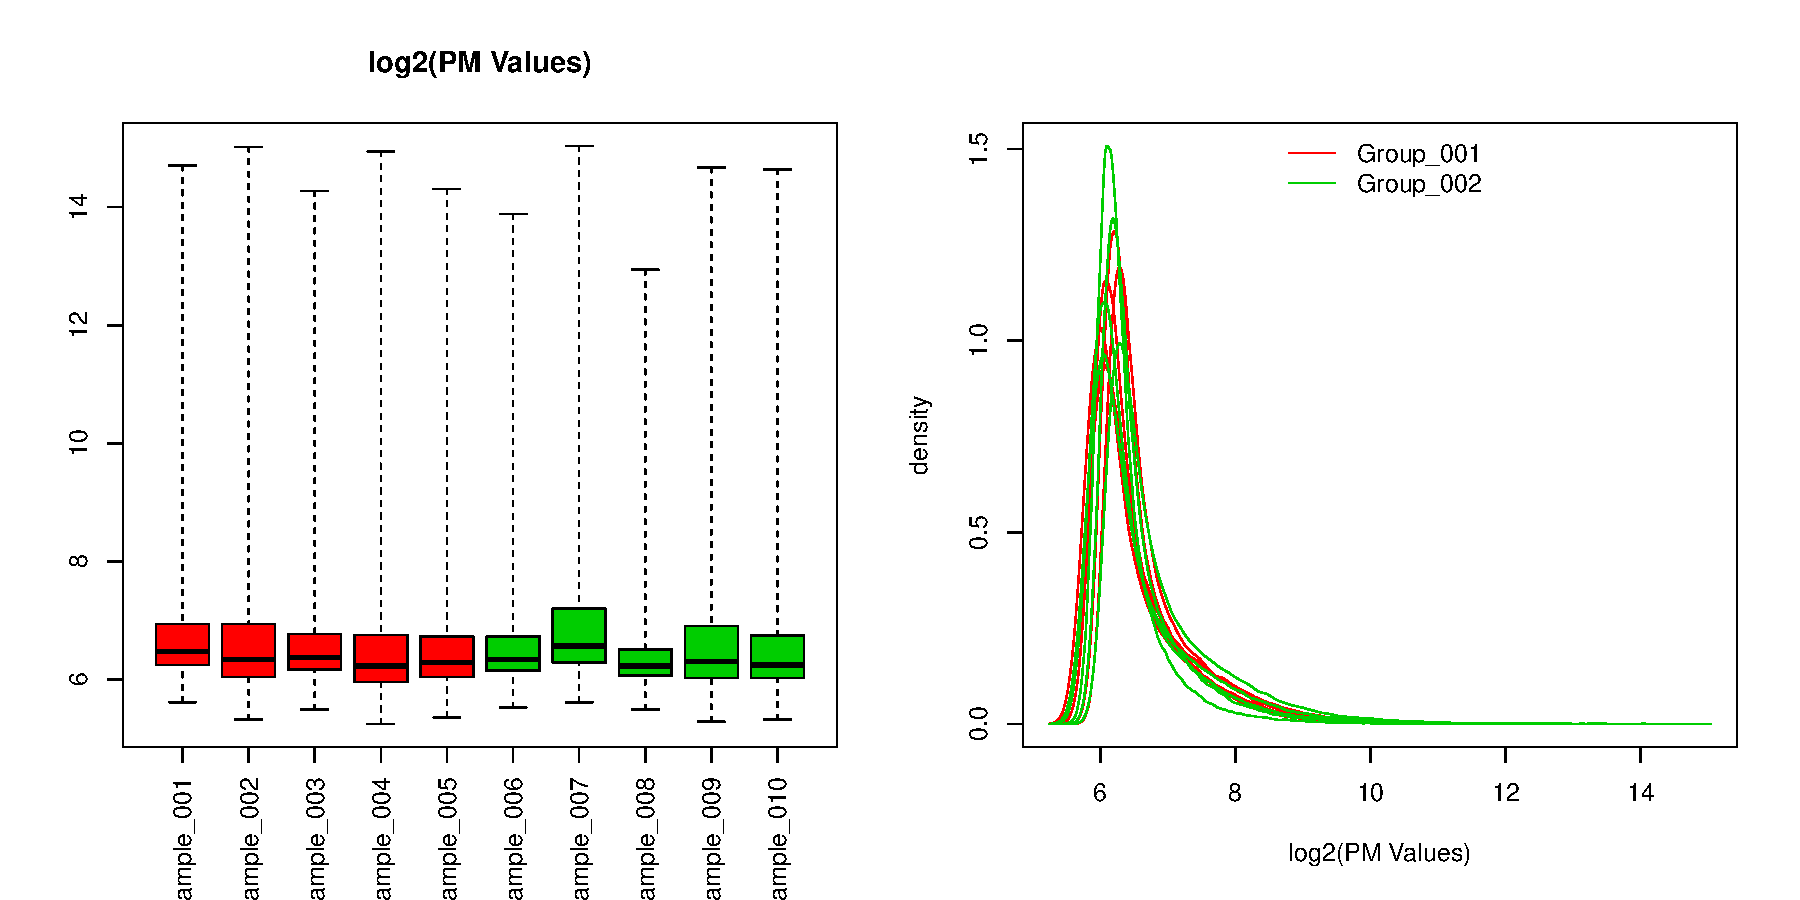
\includegraphics[width=\maxwidth]{figure/simGene-figs2-1} 

\end{knitrout}
These are the default values for the (\texttt{siga}, \texttt{sigb} 
and \texttt{sibOpt}) parameters in the \texttt{simulateGEx} function. 

To control how much technical variation is induced from the 
platform-technology, the variance hyperparameters from the sample-level 
noise (\texttt{siga}, \texttt{sigb} and \texttt{sibOpt}) can be 
controlled manually.
\begin{knitrout}
\definecolor{shadecolor}{rgb}{0.969, 0.969, 0.969}\color{fgcolor}\begin{kframe}
\begin{alltt}
\hlkwd{set.seed}\hlstd{(}\hlnum{999}\hlstd{)}
\hlstd{siga} \hlkwb{=} \hlstd{sigb} \hlkwb{=} \hlnum{1} \hlopt{*} \hlkwd{diag}\hlstd{(}\hlnum{10}\hlstd{)}
\hlstd{sigOpt} \hlkwb{=} \hlnum{1} \hlopt{*} \hlkwd{diag}\hlstd{(}\hlnum{10}\hlstd{)}

\hlstd{geneTruth} \hlkwb{<-} \hlkwd{simulateGExTruth}\hlstd{(}\hlkwc{nGenes} \hlstd{=} \hlnum{2e4}\hlstd{,} \hlkwc{nGroups} \hlstd{=} \hlnum{2}\hlstd{,}
                              \hlkwc{pDiff} \hlstd{=} \hlnum{0.05}\hlstd{,} \hlkwc{foldDiff} \hlstd{=} \hlnum{5}\hlstd{)}
\end{alltt}


{\ttfamily\noindent\itshape\color{messagecolor}{\#\# [quantroSim]: Simulating RNA transcript counts using a Poisson \\\#\#\ \ \ \ \ \ \ \ \ \  distribution with mean parameters from 0.01 to 4662.66}}\begin{alltt}
\hlstd{sim} \hlkwb{<-} \hlkwd{simulateGEx}\hlstd{(geneTruth,}  \hlkwc{GEx.platform} \hlstd{=} \hlstr{"GExArrays"}\hlstd{,} \hlkwc{nSamps} \hlstd{=} \hlnum{5}\hlstd{,}
                   \hlkwc{siga} \hlstd{= siga,} \hlkwc{sigb} \hlstd{= sigb,} \hlkwc{sigOpt} \hlstd{= sigOpt)}
\end{alltt}


{\ttfamily\noindent\itshape\color{messagecolor}{\#\# Simulating gene expression samples using the GEx.platform: GExArrays\\\#\# No PCR amplification of RNA transcript counts.}}\begin{alltt}
\hlkwd{plotGEx}\hlstd{(sim)}
\end{alltt}
\end{kframe}
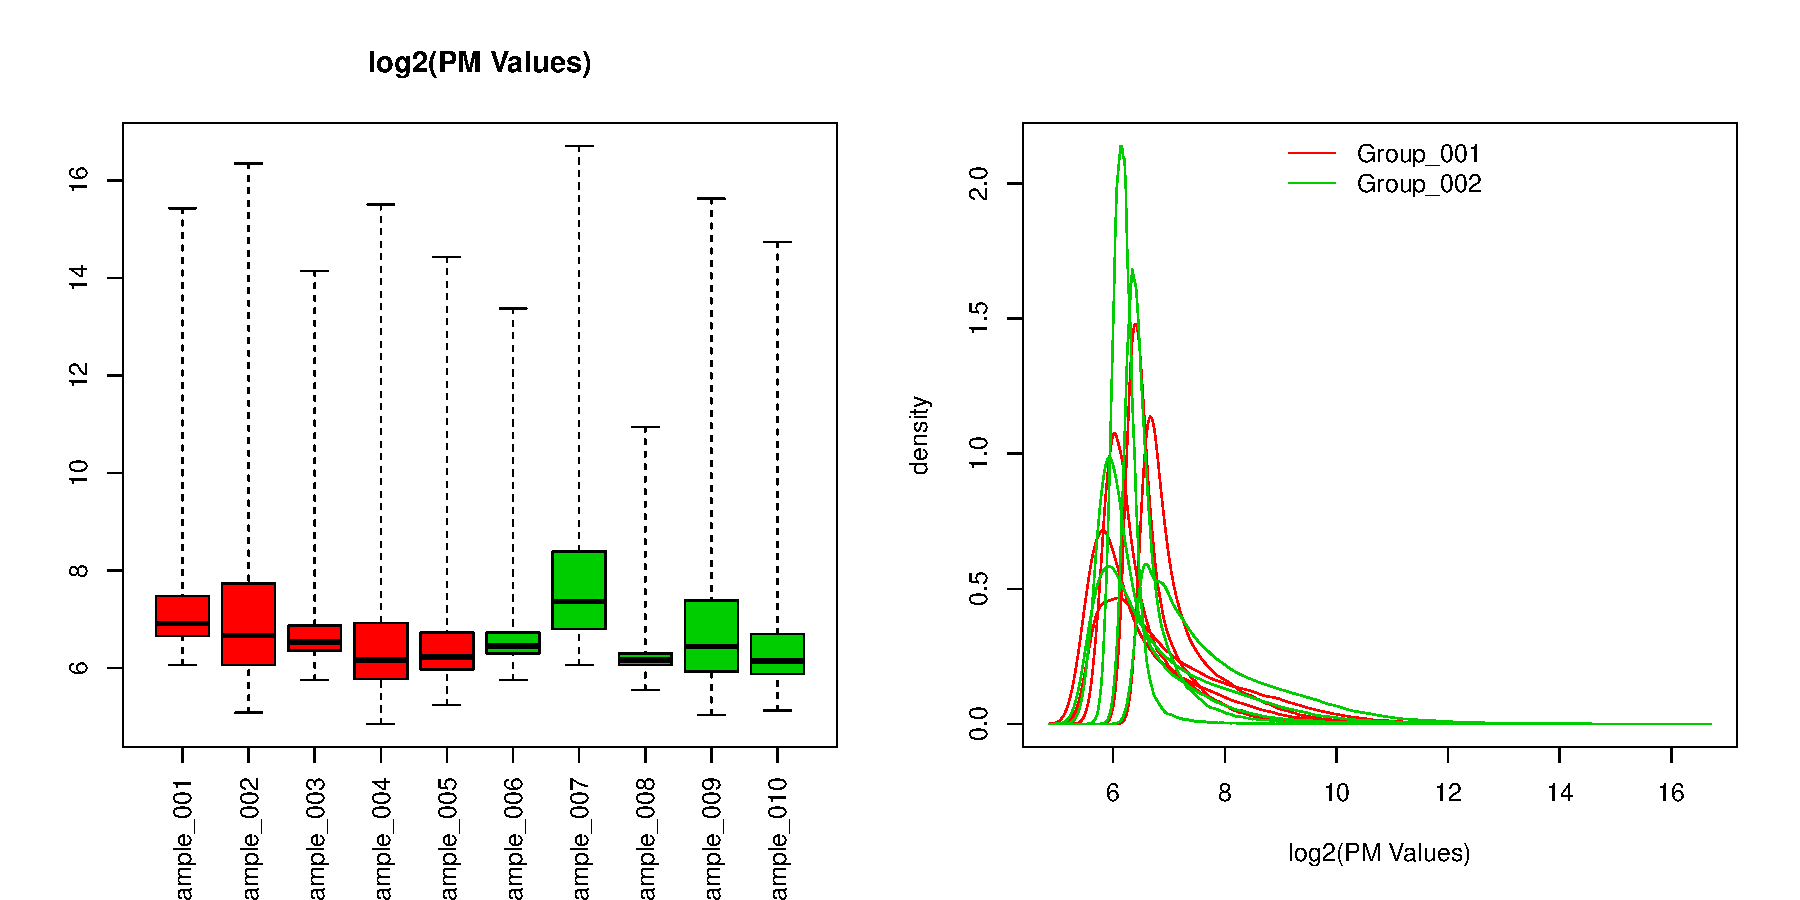
\includegraphics[width=\maxwidth]{figure/simGene-figs3-1} 

\end{knitrout}



\section{Getting Help}
For more help, open the HTML help file:
\begin{knitrout}
\definecolor{shadecolor}{rgb}{0.969, 0.969, 0.969}\color{fgcolor}\begin{kframe}
\begin{alltt}
\hlkwd{help}\hlstd{(}\hlkwc{package} \hlstd{=} \hlstr{'quantroSim'}\hlstd{,} \hlkwc{help_type} \hlstd{=} \hlstr{'html'}\hlstd{)}
\end{alltt}
\end{kframe}
\end{knitrout}


\section{SessionInfo}

\begin{knitrout}
\definecolor{shadecolor}{rgb}{0.969, 0.969, 0.969}\color{fgcolor}\begin{kframe}
\begin{alltt}
\hlkwd{sessionInfo}\hlstd{()}
\end{alltt}
\begin{verbatim}
## R version 3.1.2 (2014-10-31)
## Platform: x86_64-apple-darwin13.4.0 (64-bit)
## 
## locale:
## [1] en_US.UTF-8/en_US.UTF-8/en_US.UTF-8/C/en_US.UTF-8/en_US.UTF-8
## 
## attached base packages:
## [1] parallel  stats     graphics  grDevices utils     datasets  methods   base     
## 
## other attached packages:
## [1] quantroSim_0.0.1    Biobase_2.26.0      BiocGenerics_0.12.1 knitr_1.8          
## 
## loaded via a namespace (and not attached):
##  [1] annotate_1.44.0       AnnotationDbi_1.28.1  base64_1.1           
##  [4] beanplot_1.2          BiocStyle_1.4.1       Biostrings_2.34.0    
##  [7] bumphunter_1.6.0      codetools_0.2-9       colorspace_1.2-4     
## [10] DBI_0.3.1             digest_0.6.4          doParallel_1.0.8     
## [13] doRNG_1.6             evaluate_0.5.5        foreach_1.4.2        
## [16] formatR_1.0           genefilter_1.48.1     GenomeInfoDb_1.2.3   
## [19] GenomicRanges_1.18.3  ggplot2_1.0.0         grid_3.1.2           
## [22] gtable_0.1.2          highr_0.4             illuminaio_0.8.0     
## [25] IRanges_2.0.0         iterators_1.0.7       lattice_0.20-29      
## [28] limma_3.22.1          locfit_1.5-9.1        MASS_7.3-35          
## [31] matrixStats_0.10.3    mclust_4.4            minfi_1.12.0         
## [34] multtest_2.22.0       munsell_0.4.2         nlme_3.1-118         
## [37] nor1mix_1.2-0         pkgmaker_0.22         plyr_1.8.1           
## [40] preprocessCore_1.28.0 proto_0.3-10          quadprog_1.5-5       
## [43] quantro_1.0.0         R.methodsS3_1.6.1     RColorBrewer_1.0-5   
## [46] Rcpp_0.11.3           registry_0.2          reshape_0.8.5        
## [49] reshape2_1.4          rngtools_1.2.4        RSQLite_1.0.0        
## [52] S4Vectors_0.4.0       scales_0.2.4          siggenes_1.40.0      
## [55] splines_3.1.2         stats4_3.1.2          stringr_0.6.2        
## [58] survival_2.37-7       tools_3.1.2           XML_3.98-1.1         
## [61] xtable_1.7-4          XVector_0.6.0         zlibbioc_1.12.0
\end{verbatim}
\end{kframe}
\end{knitrout}


% \bibliography{library}


\end{document}
